\documentclass{MScthesisITEM}

% this package is just to generate text for demo-purposes
\usepackage{blindtext}


\title{Title} % The title of your assignement; NB use \newlinetitle to start a newline
\author{Vegard Stjerna Lindrup} % Your firstname and lastname
\professor{Tor Engebret Onshus} % Affiliation = ITEM for instance
%\supervisor{Firstname Lastname, Affiliation}

%% Uncomment the following in case you want subfigures; note that there will be a warning for the caption package
% \let\subcaption\undefined
% \let\subfloat\undefined
% \usepackage[bf]{caption}
% \usepackage{subcaption}

\DeclareGraphicsExtensions{.pdf,.jpg, .png}
\graphicspath{{./figs/}}
\usepackage{subcaption}
\usepackage{lscape}
\usepackage{rotating}
\usepackage{epstopdf}


\setlength\parindent{0pt} % Remove indentations.

% ---- BEGIN - Keypress illustrations ----%
\usepackage[T1]{fontenc}
\usepackage[utf8]{inputenc}
\usepackage{tikz}
\usetikzlibrary{shadows}

\newcommand*\keystroke[1]{%
  \tikz[baseline=(key.base)]
    \node[%
      draw,
      fill=white,
      drop shadow={shadow xshift=0.25ex,shadow yshift=-0.25ex,fill=black,opacity=0.75},
      rectangle,
      rounded corners=2pt,
      inner sep=1pt,
      line width=0.5pt,
      font=\scriptsize\sffamily
    ](key) {#1\strut}
  ;
}
% ---- END - Keypress illustrations ----%
% ---- BEGIN - Definition XML listings ----%
\usepackage{listings}

\usepackage{color}
\definecolor{gray}{rgb}{0.4,0.4,0.4}
\definecolor{darkblue}{rgb}{0.0,0.0,0.6}
\definecolor{cyan}{rgb}{0.0,0.6,0.6}

\lstset{
	basicstyle=\ttfamily,
	columns=fullflexible,
	showstringspaces=false,
	commentstyle=\color{gray}\upshape
}

\lstdefinelanguage{XML}
{
	morestring=[b]",
	morestring=[s]{>}{<},
	morecomment=[s]{<?}{?>},
	stringstyle=\color{black},
	identifierstyle=\color{darkblue},
	keywordstyle=\color{cyan},
	morekeywords={xmlns,version,type}% list your attributes here
}
% ---- END - Definition XML listings ----%

\usepackage{acronym} 
\acrodefplural{ROV}[ROVs]{Remotely Operated Vehicles}
\acrodefplural{AUV}[AUVs]{Autonomous Underwater Vehicles}
\acrodefplural{AIV}[AIVs]{Autonomous Inspection Vehicles}
\acrodefplural{NUI}[NUIs]{Natural User Interfaces}
\acrodefplural{LIDAR}[LIDARs]{LIght Detection And Ranging devices}
\acrodefplural{RPAS}[RPAS]{Remotely Piloted Aerial Systems}
\acrodefplural{UAV}[UAVs]{Unmanned Aerial Vehicles}

\loadglsentries{glossary}
\makeglossaries

\begin{document}
	
\selectlanguage{english}
\pagenumbering{roman}
\pagestyle{plain}

%% Only for the project; comment out the line below for the master's thesis; the front page will be generated automatically by DAIM
\titleITEM

%% Only for the master's thesis; for the project report the description is taken from It's Learning and added by the department
% \selectlanguage{english} % Change to 'norsk' if you are writing in Norwegian
\begin{titlingpage}

\noindent
\begin{tabular}{@{}p{4cm}l}
\textbf{Title:} 	& \thetitle \\
\textbf{Student:}	& \theauthor \\
\end{tabular}

\vspace{4ex}
\noindent\textbf{Problem description:}
\vspace{2ex}

Dette legges til i DAIM, og blir derfor fjernet før innlevering.
\vspace{6ex}

\noindent
\begin{tabular}{@{}p{4cm}l}
\textbf{Responsible professor:} 	& \theprofessor \\
\textbf{Supervisor:}			& \thesupervisor \\
\end{tabular}

\end{titlingpage}
\cleardoublepage

%% There must be an abstract in English, even though the main text is in Norwegian
\selectlanguage{english}
\pagestyle{empty}
\begin{abstract}
\noindent \Blindtext[5][1]
\end{abstract}
\cleardoublepage

%% Only for the master's thesis; if the main text is in English and you can write Norwegian, there must be an abstract in Norwegian as well.
\selectlanguage{norsk}
\pagestyle{empty}
\renewcommand{\abstractname}{Sammendrag}
\begin{abstract}
Robotisert vedlikehold har vært et tema i flere masteroppgaver og fordypningsprosjekter ved Institutt for teknisk kybernetikk (ITK) - NTNU over mange år. Denne oppgaven viderefører temaet, og ser nærmere på kamerabasert kartlegging og navigasjon i forbindelse med robotisert vedlikehold, samt robotisert vedlikehold generelt. Målet med oppgaven er å implementere én eller flere funksjonaliteter basert på kamerabaserte sensorer i en mobil autonom robot.  Dette gjøres ved å skaffe kunnskap om eksisterende løsninger og fremtidige behov innen robotisert vedlikehold. 

En mobil robot prototype er blitt konfigurert til å kjøre ROS (Robot Operating System), et mellomvare rammeverk som er velegnet til utvikling av robotsystemer. Systemet benytter RTAB-Map (Real-Time Appearance Based Mapping) til å kartlegge omgivelsene og en innebygget navigasjons-stack i ROS for å navigere autonomt mot enkle mål i kartet. Metoden benytter en Kinect for Xbox 360 som hovensensor, og en 2D laserskanner til både kartlegging og odometri.

Det er i tillegg utviklet fungerende konsepter for to støttefunksjoner, en Android applikasjon for fjernstyring over Bluetooth og en fjernstyringssentral (OCS) utviklet i Qt. Fjernstyringssentralen er en skjelett-implementasjon som er i stand til å fjernstyre roboten via Wifi, samt å vise video fra robotens kamera.

Testresultatene, som er inhentet fra simuleringer og testing av selve roboten, viser at roboten er i stand til å danne 3D- og 2D-kart av omgivelsene. Metoden har svakheter som er knyttet til evnen til å finne visuelle kjennemerker. Laserbasert odometri kan lures når omgivelsene er i endring, og når det er få unike kjennemerker. Videre testing har demonstrert at roboten kan navigere autonomt, men det er fortsatt rom for forbedringer. Bedre resultater kan oppnås med en ny bevegelig plattform og videre tuning av systemet.

Den endelige konklusjonen er at ROS fungerer godt som utviklingsverktøy for roboter, og at det nåværende systemet er egnet for videre utvikling. RTAB-Maps egnethet til bruk på en industriell installasjon er fremdeles usikkert, og krever videre testing.


\end{abstract}
\cleardoublepage

\selectlanguage{english}% Change to 'norsk' if you are writing in Norwegian

\renewcommand{\abstractname}{Preface}
\begin{abstract}
This thesis concludes my time as a master's student at NTNU. The last five years have been brimming with challenges and learning experiences, but I believe that the last two years have been the most rewarding by far. Both this project, and last years specialization project has fueled my interest in computer vision and robotics. Another cause for this interest is probably also due to readily available libraries and frameworks such as ROS, Qt and OpenCV.

A challenging part of the project work this semester was the openness of the problem description. Looking for, and finding tools consumed a lot of time in the initial weeks. Some ideas turned out to be blind alleys or associated with and unacceptable level of uncertainty. On the other hand, this uncertainty made the project more interesting, and it could be that I never would have come around to use ROS without it.

To students who are considering to continue working on this project, I would recommend that they get a solid background in use of ROS, perhaps by taking part in the subject TTK8, taught by Amund Skavhaug.
\newline\newline\newline
Vegard Stjerna Lindrup
\newline\newline
\today

\end{abstract}
\cleardoublepage

% similarly you may add a separate acknowledgments page
\renewcommand{\abstractname}{Acknowledgments}
\begin{abstract}
This thesis, and the obtained project results would not have been possible without help from student colleagues, friends and support from the Department of Engineering Cybernetics. 

I would first like to thank my project supervisor, Professor Tor Onshus of the Department of Engineering Cybernetics at NTNU, for allowing me to work on such an open and interesting topic, and for providing valuable advice and guidance through the two last semesters. He has been quick to respond to problems with the project, and gave me a much needed sense of urgency when the project was lagging far behind schedule in march.

Among my student colleagues, Eirik Wold Solnør, Vegard Blomseth Johnsen and Henrik Rudi Haave have been particularly helpful during testing sessions and for video documentation. Over the last two semesters, Ole Magnus Siqveland and I have used the same robot platform for our projects. Through good collaboration, we found a hardware setup that worked for both of us; a new shelf structure with compartments for the various hardware components.

I would like to thank the foreman, Terje Haugen, and apprentice Daniel Bogen at the mechanical workshop for building the new compartments and frames for the robot used in this thesis. Many thanks goes to the employees at the electronics workshop for allowing me to borrow tools and equipment, and providing some hints and tips. 

I am very grateful to my parents and Andrea Myklebust for supporting me through the years at NTNU. Thank you!

Sincerely,\\
Vegard Stjerna Lindrup


\end{abstract}
\cleardoublepage

\tableofcontents*
\cleardoublepage

\addcontentsline{toc}{chapter}{List of Acronyms}
\cleardoublepage

%% include if relevant
\listoffigures
\cleardoublepage

%% include if relevant
\listoftables
\cleardoublepage

\chapter*{List of Acronyms}
\addcontentsline{toc}{chapter}{List of Acronyms}
\begin{acronym}
\acro{AI}{Artificial Intelligence}

	\acro{AIV}{Autonomous Inspection Vehicle}

    \acro{CLM}{Concurrent Localization and Mapping}

	\acro{CP}{Cathodic Protection}

	\acro{DRC}{DARPA Robotics Challenge}

    \acro{Fraunhofer IPA}{Fraunhofer Institute for Manufacturing Engineering and Automation}

	\acro{GUI}{Graphical User Interface}

	\acro{HMI}{Human-Machine Interaction}
	
	\acro{HSE}{Health, Safety and Environment}

	\acro{IFR}{International Federation of Robotics}
	
	\acro{IO}{Integrated Operations}

	\acro{ISS}{International Space Station}
	
	\acro{ITK}{Department of Engineering Cybernetics}

	\acro{LIDAR}{LIght Detection And Ranging}

	\acro{MIMROex}{Mobile Inspection and Monitoring Robot, experimental}

    \acro{NCS}{Norwegian Continental Shelf}

	\acro{NDT}{Non-destructive Testing}

	\acro{MIT}{Massachusetts Institute of Technology}

	\acro{NUI}{Natural user interface}

	\acro{OCS}{Operator Control Station}
	
	\acro{OG}[O\&G]{Oil \& Gas}
	
	\acro{PCL}{Point Cloud Library}

	\acro{PR}{Personal Robot}
	
	\acro{PWM}{Pulse Width Modulation}
	
	\acro{RBI}{Risk Based Inspection}

	\acro{ROS}{Robot Operating System}

	\acro{ROV}{Remotely Operated Vehicle}
	
	\acro{RPAS}{Remotely Piloted Aerial System}

	\acro{RTAB-Map}{Real-Time Appearance-Based Mapping}

	\acro{SDF}{Simulation Description Format}
	
	\acro{SIFT}{Scale-invariant feature transform }
	
	\acro{SIM}{Structural Integrity Management}

	\acro{SLAM}{Simultaneous Localization And Mapping}
	
	\acro{SSD}{Solid State Drive}
	
	\acro{SURF}{Speeded Up Robust Features}

	\acro{STAIR}{Stanford AI Robot}
	
	\acro{UAV}{Unmanned Aerial Vehicle}

	\acro{URDF}{Unified Robot Description Format}
	
	\acro{VR}{Virtual Reality}
\end{acronym}

%% include if relevant
\listofalgorithms
\addcontentsline{toc}{chapter}{List of Algorithms}
\cleardoublepage

% include if relevant
%\printglossary[title=List of Symbols, style=long]
%\cleardoublepage
%\glsaddall[]

% include if relevant
%\printglossary[title=List of Acronyms,type=\acronymtype] % prints just the list of acronyms
%\cleardoublepage

\pagenumbering{arabic}
\pagestyle{ruled}
%\chapter{Example}
\label{chp:example} 

Here is an example of how to use acronyms such as \gls{ntnu}. The second time only \gls{ntnu} is shown and if there were several you would write \glspl{ntnu}. And here is an example\footnote{A footnote} of citation~\cite{Author:year:XYZ}. 

\Blindtext[3][1]

\begin{figure}
\centering
% dummy figure replacement 
\begin{tabular}{@{}c@{}}
\rule{.5\textwidth}{.5\textwidth} \\
\end{tabular}
\caption{\label{fig:example}A figure}
\end{figure}

\section{First section}\label{sec:first_section}

\subsection{First subsection with some \texorpdfstring{$\mathcal{M}ath$}{Math} symbol}\label{sec:first_ssection}

\blindtext
\begin{itemize}[topsep=-1em,parsep=0em,itemsep=0em] % see http://mirror.ctan.org/macros/latex/contrib/enumitem/enumitem.pdf for details about the parameters
 \item item1
 \item item2
 \item ...
\end{itemize}

\subsection{Mathematics}

\blindmathtrue
\blindtext

\begin{proposition}\label{def:a_proposition}
A proposition... (similar environments include: theorem, corrolary, conjecture, lemma)

\end{proposition}

\begin{proof}
\vspace*{-1em} % Adjust the space when parskip is set to 1em
And its proof.
\end{proof}

\begin{table}
\caption{\label{tab:example}A table}
\centering
\begin{tabular}[b]{| c | c | c | c | c |}
\hline
a & b & c & d & e \\ \hline
f & g & h & i & j \\ \hline
k & l & m & n & o \\ \hline
p & q & r & s & t \\ \hline
u & v & w & x & y \\ \hline
z & æ & ø & å &   \\ \hline
\end{tabular} 
\end{table}

\subsection{Source code example}

% \floatname{algorithm}{Source code} % if you want to rename 'Algorithm' to 'Source code'
\begin{algorithm}[h]
  \caption{The Hello World! program in Java.}
  \label{hello_world}
  % alternatively you may use algorithmic, or lstlisting from the listings package
  \begin{verbatim}
  
class HelloWorldApp {
  public static void main(String[] args) {
    //Display the string
    System.out.println("Hello World!");
  }
}
\end{verbatim}
\end{algorithm}

You can refer to figures using the predefined command like \fref{fig:example}, to pages like \pref{fig:example}, to tables like \tref{tab:example}, to chapters like \Cref{chp:example} and to sections like \Sref{sec:first_section} and you may define similar commands to refer to proposition, algorithms etc.

%% include here the other chapters

\chapter{Introduction}
\label{chp:introduction} 

Introduction
\section{About the Thesis}

\section{Mobile Robotic Maintenance}

\section{Implementation Overview}

\section{Thesis Structure}
%\chapter{Task Outline and Planning}
\label{chp:TaskOutlineAndPlanning}

\section{Introduction}

The original problem description given at the beginning of this semester is very open. A significant part of the project is oriented towards 

\section{Task definition}

\section{Specification}

\section{Planning}

\subsection{Work Breakdown Structure}
\chapter{Robotic Maintenance on Topside Offshore Platforms}
\label{chp:maintenance}

\section{Introduction}

This project is a small step towards a larger long-term goal concerning robotic maintenance on topside offshore installations. This chapter puts the implementation described in chapter \ref{chp:implementation} into the context of the long-term goal. 

Over the last decade, the \ac{OG} industry has shown an increased interest in the potential benefits of automating the normal operation of remote offshore installations. Some satellite platforms, such as Sleipner B are already unmanned during normal operation, and the more recent Valemon platform is planned to become normally unmanned as well. It is now clear that robotics has several potential applications in process plants, and particularly in remote \ac{OG} installations. It is, however, difficult to predict how and to what extent robots will be applied in plant automation as other innovative solutions may arise\cite{statoil_ubemannet}\cite{subsea_konkurranse}\cite{E24}. Current research on plant automation is mainly motivated by two factors\cite{AutonomousOG} \cite{StepwiseApproachToRobotics}:

\begin{itemize}
	\item \textbf{HSE} - Reduced risk exposure for personnel and environment. 
	\item \textbf{Efficiency} - Accomplish more with less effort, resources and time. This means cost reduction by keeping downtime to a minimum with the least amount of effort.
\end{itemize} 

An additional overarching driving factor is that \ac{OG} fields are becoming more difficult to reach. As \ac{OG} fields in shallow waters are depleted, production is moved to deeper waters. This complicates the extraction process and reduces the profit margin. A solution to this challenge is to increase efficiency through further automation. 

This chapter provides a brief introduction to how topside maintenance is performed today, how these maintenance tasks could be robotized. The chapter is concluded with a brief discussion on how well modern robotics is suited for the task. 

%\subsection{Potential Maintenance Tasks}

%Hidden failure modes: PFD: What is the probability that a device (Fire detector, shut down valve, etc.) will fail when needed? 
%Solution: Periodic maintenance.

\section{Robotizing Offhsore Maintenance}
\label{sec:robotizing_offhsore_maintenance}
%In light of the factors listed earlier, maintenance and service robots will be designed with the following goals in mind\cite{AutonomousOG}:

Recent research projects, concept labs and prototypes seem to focus on a solution where stationary or mobile robots serve in a supporting role in parallel to the dedicated process automation systems\cite{StepwiseApproachToRobotics}\cite{sintef_robot_consept}\cite{graf2008mobile}\cite{6094661}. 

A feasibility study performed by researchers from \ac{Fraunhofer IPA}\cite{6094661} identified several topside production tasks and ranked them according to their resource demand. 
%Table \ref{tab:tasks} shows the ranked tasks based on a preselected installation. While all tasks would benefit from ''robotizing'',  
Based on the identified tasks, the study went on to describe a set of specific tasks, and then assess how easy or hard it would be to ''robotize'' these tasks. Table \ref{tab:tasks_capabilities} associates a set of tasks with different robot categories, as well as how easy or hard the process of ''robotizing'' the activity is expected to be. The difficulty levels are described with the letters ''A'' through ''D'', where  ''A'' is described as of the shelf robotics, which makes ''robotizing'' easy. Activities associated with the letter ''D'' on the other hand, cannot be be ''robotized'' with either current or near future technology even if doing so would be beneficial \cite{6094661}. Note that the paper in question is from 2011, and the difficulty of these tasks may have changed. This is particularly true in the domain of visual sensors, given the bloom of accessible 3D sensor technology and research over the last decade. Some further elaboration on inspection activities and environmental considerations is given in the next subsection. 

\begin{table}
\centering
\begin{tabular}{ |p{2cm} p{3cm} p{5cm}| }
\hline
\multicolumn{3}{|c|}{Robot Applications Including Categorization}\\
\hline\hline
Category & Robot & Robot Task/Activity Description \\ 
\hline
B & Pipeline rigging robot & To autonomously load and offload pigs into pipelines. \\
C & Boat handling robot < 500 kg & To transfer personnel and loads below 500 kg to and from boats.\\
D & Boat handling robot > 500 kg & To transfer loads above 500 kg to and from boats.\\
\hline
B & Mobile universal service robot version 1 & To perform ''buddy'' roles; carrying, holding, lifting, personal safety monitoring etc. \\
C & Mobile universal service robot version 2 & To autonomously perform task not involving manipulation of the process or facilities.\\
D & Mobile universal service robot version 3 & To autonomously perform tasks involving manipulation of the process or facilities. \\
D & Treatment/Inspection robot & To autonomously perform inspection/treatment(painting) tasks of structures/vessels or facilities.\\
\hline
A & Domestic service robot & To autonomously perform floor cleaning, catering, laundry handling, storage handling and logistics activities. \\
\hline\hline 
\end{tabular}
\caption{Some tasks with potential to be ''robotized'', and the corresponding robot category\cite{6094661}.} 
\label{tab:tasks_capabilities}
\end{table}

The feasability study from \cite{6094661} suggests five tasks that will have a high impact on \ac{HSE} and efficiency:
\begin{itemize}
\item Monitoring of gauges and meters
\item (Visual) inspection of remote operated valves
\item Acoustic inspection
\item Inspection of equipment for leakage
\item Maintenance of gas and fire sensors
\end{itemize}

Recovery scenarios is another area of application for offshore robots. As explained in \cite{AutonomousOG}, a robot could be used to handle hazardous events that will lead to an evacuation of platform personnel. The robot could be a valuable tool in containing the hazardous situation quickly, thus reducing production downtime. 

\cite{StepwiseApproachToRobotics} from ABB suggests a stepwise approach toward robotization. The suggested approach is to break each concept and problem down into specific manageable tasks, before allowing the developed solutions to mature by exposing them to increasingly realistic test scenarios. Another path towards robotization corresponds to the difficulty assessments and classifications in table \ref{tab:tasks_capabilities}\cite{graf2008mobile}. This roadmap starts with the bare necessities, e.g. tele-operation, ATEX certifications and safety. This will provide the foundation for developing inspection or surveillance robots, before the complexity can be increased by allowing robots to interact with and manipulate the processes. The end-goal is of course a fully autonomous maintenance system capable of operating the process itself\cite{graf2008mobile}.

%\begin{table}[h!]
%\centering
%\begin{tabular}{ |p{5cm} p{2cm} p{2.5cm} | }
%\hline
% \multicolumn{3}{|c|}{Production Operation Activities} \\
% \hline\hline
% Task & Annual Man Hours & Frequency of Operations\\
% \hline
% Gas compression system operation & 4079    &Daily \\
% Ops checks \& logging & 2350 & Daily\\
% Safety Checks & 1982 & Weekly \\
% Sampling and top-up (glycol, condensate, jet A1)& 1125  & Daily\\
% Chemical Injection \& Handling & 814  & Daily   \\
% Deluge valve system & 819  & Monthly \\
% Supply \& crew boat handling & 568 & Weekly \\
% Materials handling and ordering & 446 & Daily \\
% Helicopter refuelling & 208 & weekly (?) \\
% Helicopter handling & ? & 2 days (daily?) \\
% Sump content clearance & 129 & Weekly \\
% Well testing & 79 & Daily \\
% Diesel/water bunkering & 52 & 2 Weekly \\
% First aid painting & ? & As required \\
% Pigging activities & 40 & Monthly \\
% \hline\hline
%\end{tabular}
%\label{tab:tasks_ranked}
%\caption{Identified and ranked production operation activities \cite{6094661}. Question marks and parenthesis are intentional.} 
%\end{table}



\subsection{Structural Maintenance and Environmental Considerations}

\subsubsection{Corrosion}

Offshore installations are regularly, if not continuously, exposed to harsh weather conditions in the form of wind and seawater. Presence of seawater, either through direct contact or in the form of drops and vapor, forms a very corrosive environment. The offshore and marine environment is classified as the most corrosive environment in ISO 12944\cite{ElReedy2012383}. It is essential to provide countermeasures to ensure safe and reliable operation over the lifetime of the installation. Common corrosion prevention methods are\cite{ElReedy2012383}:

\begin{itemize}
	\item Sacrificial Anodes.
	\item \ac{CP} in the form of a DC-current.
	\item Protective coating.
\end{itemize} 

In terms of maintenance, the sacrificial anodes can be subjected to periodic inspections and replacements, which could be done by a robot. \ac{CP} can more easily be implemented with automated self tests, and should normally not require any inspections and maintenance\cite{ElReedy2012383}. Application of protective coating should ideally be applied in the controlled environment of a workshop. If protective coating is to be applied at sea, one should strive to make the conditions as favourable as possible. 

\subsubsection{Structural Fatigue}

Waves, wind, water currents and other forces subject offshore installations to structural stress. To keep the offshore installations from failing in these conditions, they may be subjected to a \ac{RBI} regime. In brief, \ac{RBI} is a strategy where inspection and maintenance programs are developed based on which risk factors an installation is exposed to. In an automated maintenance program, an autonomous robot could perform inspections of the structure and generate reports based on risk factors such as\cite{ElReedy2012563}:

\begin{description}
\item[Marine growth at sea level] Marine growth will increase the diameter of supporting legs at sea level, thus increasing structural loads caused by waves, wind and water currents. 
\item[Corrosion] Assess the seriousness of a corrosion attack through \ac{NDT}.
\item[Scour] Scour around the platform legs could reduce a platforms ability to withstand structural loads. This is only applicable to non-floating installations.
\end{description}

A maintenance expert can then plan a maintenance campaign based on data from the robot in combination with knowledge on the platforms design, age and exposure to the environment.

\subsection{Production-specific Hazards}

\ac{OG} production has several inherent hazards, and an unwanted incident may have serious implications for \ac{HSE} and production uptime. The Piper Alpha incident serves as a worst case example of the consequences of an explosive ignition of a hydrocarbon leak followed by an escalating fire. This section will briefly discuss some of the most significant hazards on an offshore oil and gas production plant.

%\begin{description}
%\item[Hydrocarbon leaks - ] 

%\item[Fire - ]  

%\item[Explosions -]
%\end{description}

\subsubsection{Hydrocarbon leaks}

Hydrocarbon leaks do occur on a regular basis. Over a four year period from 2006 to 2010, seven leaks larger than $1 kg/s$ of either oil or gas/two-phase occurred in the Norwegian sector. No such leaks have ignited on the \ac{NCS} since 1992. Of all the leaks which occurred in the same area, \ac{NCS}, the majority was caused by human intervention\cite{Vinnem2014}. This could imply that a reliable robotic system may reduce the number of leaks.

\subsubsection{Fire}

Critical fire loads\footnote{Fire load can be defined as the amount of combustible material in a given area (Ref. \url{https://en.wiktionary.org/wiki/fire_load}).} on offshore facilities are usually caused by uncontrolled flow of hydrocarbons. The most serious of such releases is a blow-out. Risk reducing measures focus on four areas\cite{Vinnem2014}: 

\begin{description}
\item[Leak prevention - ] Use equipment and assembly methods which minimize risk.

\item[Leak detection - ]  Fire \& gas detection, emergency shut-down systems and blowdown systems.

\item[Ignition prevention -] Inspection and maintenance and Ex-approved equipment.

\item[Escalation protection  -] Installation layout and sectioning. Fire and gas protection systems.
\end{description}


\subsubsection{Explosions}

Explosion protection is usually built into the equipment and structure. In \cite{Vinnem2014}, there are no obvious ways a robot could provide additional explosion beyond e.g. leak detection, inspection and maintenance. 

\subsection{Implications for Robot Design}

A mobile robot operating on a normally unmanned platform in a harsh environment, implies that it is subjected to many of the same design philosophies that apply to subsea equipment. 

Because of the risk of explosive atmospheres in an offshore production environment, an offshore robot operating under EU or EEA legislation will also be subject to the ATEX (ATmosphères EXplosibles) directive. Such a robot will most likely carry ignition sources such as batteries packed with energy and perhaps even welding equipment. A central ATEX requirement is to perform a risk assessment. As outlined by ATEX 2014-34-EU Guidelines\cite{ATEX_guidelines}, such a risk assessment is usually performed in four steps:

\begin{description}
\item[1. Hazard identification \-] What can go wrong? Identify possible ignition sources, and the probability of explosive atmospheres.
\item[2. Risk estimation \-] Estimate the probability of an unwanted occurrence (e.g. an explosion), and the associated consequences.
\item[3. Risk evaluation \-] Evaluate the identified risk in context of acceptable risk, and decide if the design should be altered or if additional barriers should be installed. Barriers could either mitigate the consequences of an explosion, or reduce the possibility of ever having an explosion.
\item[4. Risk reduction option analysis \-] Identify possible risk reduction measures, e.g. barriers and design changes. A cost-benefit analysis can be performed in accordance with the ALARP-principle. 
\end{description}

The on-board embedded computer hardware and software should be designed for robustness, fault tolerance and endurance. If a failure occurs, corrective actions will most likely be both difficult and expensive. Resistance to corrosion and toxic environments should also be taken into account.

Other design choices, e.g. the shape, size and equipment must fit the robots purpose. A source of guidelines for a mobile robot can draw upon case studies such as e.g. \cite{graf2008mobile}.

\section{Robotic Maintenance Today}
 
\subsection{Trends and Potential}
 
The typical pre-programmed assembly robots still dominate the robotic market. They are usually found in manufacturing plants and large scale production facilities\cite{ifr_statistics}, e.g. the automotive industry, where they perform dull, tedious tasks much faster and with higher accuracy than people. A notable trend in modern robotics is increased human-robot collaboration\cite{cobotsEurope}. Many new robots are being built for the human workspace, both in terms of safety and collaborative functionality. This trend is a step along the way of moving robots out of the controlled environment of a factory floor, and into the real world where a high degree of autonomy is required.

A report by Metra Martech\cite{metraMartechGorle}, a market research firm referenced to by \ac{IFR}\footnote{http://www.ifr.org/robots-create-jobs/}, points to three areas with a high potential for robotic applications:

\begin{itemize}
	\item Dangerous jobs, e.g. handling dangerous materials or work in high risk environments.
	\item Jobs that are economically infeasible in a high wage economy.
	\item Work which is impossible or highly inconvenient for humans, e.g. space exploration, subsea maintenance or assembly of heavy components.
\end{itemize}

All of these factors motivate the development of robots for autonomous robotic maintenance. 

\subsection{Subsea Maintenance and Inspection}

\begin{wrapfigure}{r}{0.5\textwidth}
	\vspace{-20pt}
	\begin{center}
		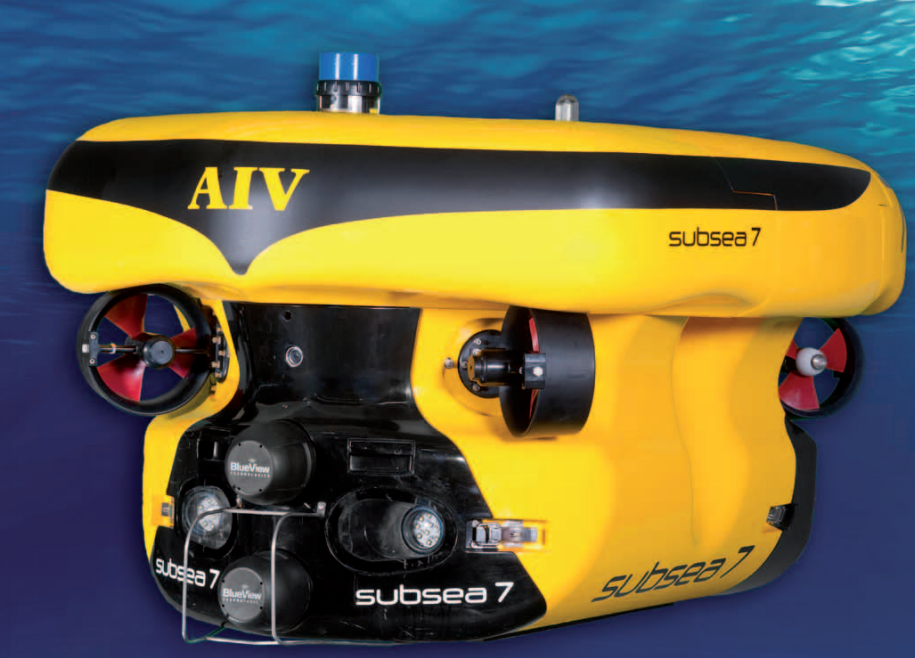
\includegraphics[width=0.48\textwidth]{subsea7AIV}
	\end{center}
	
	\caption{Subsea 7's AIV. This is the first commercial autonomous inspection vehicle for subsea operations \cite{pressAIV}}
	%\vspace{-20pt}
\end{wrapfigure}

Subsea maintenance is perhaps the field that have seen the greatest advancements in autonomous inspection and maintenance. As offshore installations are moved to the seabed, maintenance and inspection has become a significant challenge. This has resulted in a widespread use of \acp{ROV}. Recent developments in other fields, e.g. computer vision, human-robot collaboration and machine learning, has resulted in new \acp{AIV} and \acp{AUV} capable of performing inspection and simple maintenance tasks autonomously\cite{subseaAIV}\cite{Ridao2015227}. A driving factor behind the transition from \acp{ROV} to \acp{AUV} is cost reduction through increased offshore campaign efficiency.

\subsection{Disaster Response}

\begin{wrapfigure}{r}{0.5\textwidth}
	%\vspace{-20pt}
	\begin{center}
		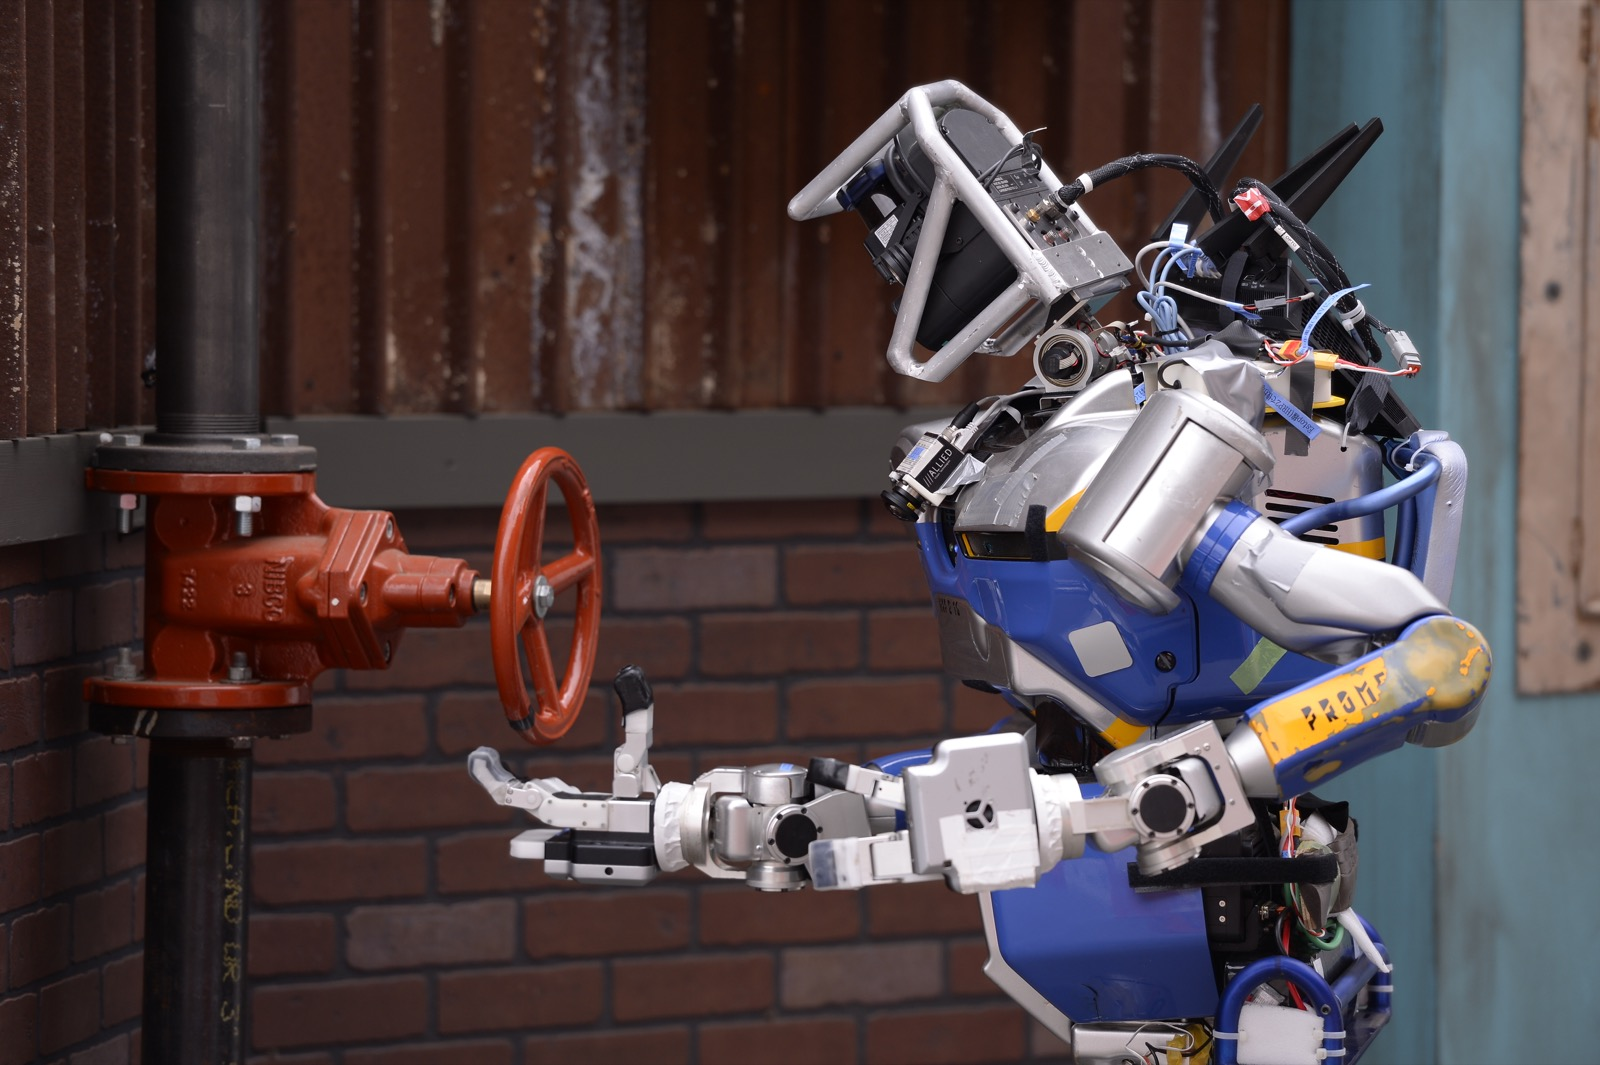
\includegraphics[width=0.48\textwidth]{HRP2_valve}
	\end{center}
	
	\caption{Team HRP2-Tokyo's robot turning a valve during DARPA Robotics Challenge 2015 (Image credits: DARPA Robotics Challenge)}
	%\vspace{-20pt}
\end{wrapfigure}

Robots in disaster response, relief and recovery solve many of the same problems faced by maintenance robots. Disasters, such as the tsunami which struck Japan in 2011, proved that much work needs to be done, both in terms of technical capabilities and logistical issues related to deployment and response times. The tsunami resulted in three core meltdowns at the Fukushima Daiichi Nuclear Power plant\cite{fukushima_report}.

Many of the robots which were deployed at the Fukushima Power Plant were already ageing, and the operators had to receive training before deployment, thus increasing the response time\cite{doi:10.1108/01439911211249715}. A paper from Japan Atomic Energy Agency\cite{doi:10.1108/01439911211249715} highlights how the lack of stakeholder involvement could have been the cause of long response times. The same paper points out that the robots were developed for the sake of development, and not with emergency response as the main purpose\cite{doi:10.1108/01439911211249715}. 

\ac{DRC}\cite{DRC} was launched in response to the Fukushima disaster of 2011. The purpose of the competition is to accelerate innovation, research and development in robotics for disaster response in cases where humans cannot operate. Some of the tasks the competitors faces in 2015 include valve turning, traversing rubble and driving a vehicle through a course before egressing out of the vehicle.

\subsection{Topside Offshore and Onshore Robotic Maintenance}

Today, autonomous and teleoperated inspection and maintenance is usually only found at subsea installations. Topside installations on the other hand are still maintained and inspected manually, with some notable exceptions. Small \acp{UAV} or \acp{RPAS} have become commonplace and accessible to all over the last decade. There are currently \ac{RPAS} systems which are being used for visual inspection of inaccessible structural parts such as flare stacks or the exterior of oil rigs.

Some notable contributors to the field of robotic maintenance for \ac{OG} include ABB, \ac{Fraunhofer IPA}, Sintef ICT\cite{sintef_robot_consept} and NREC  at  Carnegie
Mellon University. 

NRECs contribution, Sensabot, is a remotely operated inspection robot designed for harsh and remote environments\cite{deploymentsensabot}. It is not designed to be autonomous, but rather as a tool to move personnel from hazardous environments to safe remote control rooms. Sensabot mark II will be certified for zone 1 explosive environments. This year (2016), the plan is to test the robot on site at the Kashagan field in Kazakhstan\cite{peerless2016robot}.

\begin{wrapfigure}{l}{0.45\textwidth}
	%\vspace{-20pt}
	\begin{center}
		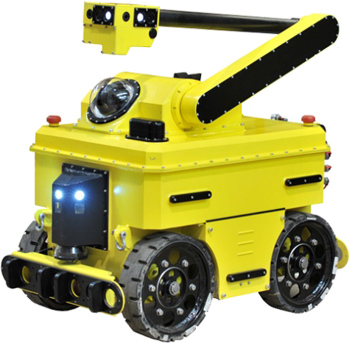
\includegraphics[width=0.42\textwidth]{sensabot}
	\end{center}
	
	\caption{An early version of the maintenance robot ''Sensabot'', developed by National Robotic Engineering Center (NREC) (Image credits: NREC)}
	\vspace{-20pt}
\end{wrapfigure} 

\ac{Fraunhofer IPA}\footnote{http://www.ipa.fraunhofer.de/en.html} has developed a robot, called \ac{MIMROex}. \ac{MIMROex} has capabilities which are quite similar to the prototype used during the work on this thesis. \ac{MIMROex} is equipped with a camera for visual inspections as well as microphones, vibration and sensors for fire and gas detection. It is also certifiable in accordance with the explosion protection standard IEC 60079\cite{MIMROex}. \ac{Fraunhofer IPA} has put great emphasis on field testing on actual offshore installations.

Both ABB and SINTEF ICT have developed lab facilities to test various concepts for robotic maintenance. Both facilities use non-mobile or semi mobile (gantries) robots which utilize a rich set of inspection and manipulation tools, as well as \ac{HMI} equipment for remote operation and control. The two research communities differ in that ABB has tested their solutions in real environments, which subjects their solution to ATEX requirements and an extensive risk management regime\cite{StepwiseApproachToRobotics}. SINTEF has a notable list of contributions to computer vision and 3D camera optics\footnote{http://www.sintef.no/en/information-and-communication-technology-ict/optical-measurement-systems-and-dataanalysis/}, and some of this research is geared towards inspection and maintenance. An example of this is a robot concept for replacing a battery in a wireless sensor by using 3D object detection\cite{transeth2010robotic}.

Another effort towards robotic maintenance is the ARGOS challenge (Autonomous Robot for Gas and Oil Sites). The purpose of the challenge is to promote innovation, understanding and awareness towards robotic maintenance of \ac{OG} sites in harsh environments\cite{ARGOS}\cite{AutonomousOG}.
\chapter{Background Theory}
\label{chp:theory} 


\section{Robotic Maintenance of Industrial Installations}

\subsection{Introduction}

This project is a small step towards a larger long-term goal concerning robotic maintenance on topside offshore installations. This section puts the following background theory, and the implementation described in chapter \ref{chp:implementation}, into the context of the long-term goal. 

This section will introduce how topside maintenance is performed today, how these maintenance tasks could be robotised. The section is concluded with a discussion on how well modern robotics is suited for the task. 

\subsection{Potential Maintenance Tasks}

Hidden failure modes: PFD: What is the probability that a device (Fire detector, shut down valve, etc.) will fail when needed? 
Solution: Periodic maintenance.

\subsection{Which Tasks Can Be Robotised?}

%In light of the factors listed earlier, maintenance and service robots will be designed with the following goals in mind\cite{AutonomousOG}:

Over the last decade, the \ac{OG} industry has shown an increased interest in the potential benefits of automating the normal operation of remote offshore installations. It is now clear that robotics has several potential applications in process plants, and particularly in remote \ac{OG} installations. Current research on plant automation is mainly motivated by two factors\cite{AutonomousOG} \cite{StepwiseApproachToRobotics}:

\begin{itemize}
	\item \textbf{HSE} - Reduced risk exposure for personnel and environment. 
	\item \textbf{Efficiency} - Accomplish more with less effort, resources and time. This means cost reduction by keeping downtime to a minimum with the least amount of effort.
\end{itemize} 

An additional overarching driving factor is that \ac{OG} fields are becoming more difficult to reach. As \ac{OG} fields in shallow waters are depleted, production is moved to deeper waters. This complicates the extraction process and reduces the profit margin. A solution to this challenge is to increase efficiency through further automation.

\begin{table}
\centering
\begin{tabular}{ |p{2cm} p{3cm} p{5cm}| }
\hline
\multicolumn{3}{|c|}{Robot Applications Including Categorization}\\
\hline\hline
Category & Robot & Robot Task/Activity Description \\ 
\hline
B & Pipeline rigging robot & To autonomously load and offload pigs into pipelines. \\
C & Boat handling robot < 500 kg & To transfer personnel and loads below 500 kg to and from boats.\\
D & Boat handling robot > 500 kg & To transfer loads above 500 kg to and from boats.\\
\hline
B & Mobile universal service robot version 1 & To perform ''buddy'' roles; carrying, holding, lifting, personal safety monitoring etc. \\
C & Mobile universal service robot version 2 & To autonomously perform task not involving manipulation of the process or facilities.\\
D & Mobile universal service robot version 3 & To autonomously perform tasks involving manipulation of the process or facilities. \\
D & Treatment/Inspection robot & To autonomously perform inspection/treatment(painting) tasks of structures/vessels or facilities.\\
\hline
A & Domestic service robot & To autonomously perform floor cleaning, catering, laundry handling, storage handling and logistics activities. \\
\hline\hline 
\end{tabular}
\caption{Some tasks with potential to be ''robotized'', and the corresponding robot category\cite{6094661}.} 
\label{tab:tasks_capabilities}
\end{table}

A feasibility study performed by researchers from \ac{Fraunhofer IPA} identified several topside production tasks and ranked them according to their resource demand. 
%Table \ref{tab:tasks} shows the ranked tasks based on a preselected installation. While all tasks would benefit from ''robotizing'',  
Based on the identified tasks, the study went on to describe a set of specific tasks, and then assess how easy or hard it would be to ''robotize'' these tasks. Table \ref{tab:tasks_capabilities} associates a set of tasks with different robot categories, as well as how easy or hard the process of ''robotizing'' the activity is expected to be. The difficulty levels are described with the letters ''A'' through ''D'', where  ''A'' is described as of the shelf robotics, which makes ''robotizing'' easy. Activities associated with the letter ''D'' on the other hand, cannot be be ''robotized'' with either current or near future technology even if doing so would be beneficial \cite{6094661}. Note that the paper in question is from 2011, and the difficulty of these tasks may have changed. This is particularly true in the domain of visual sensors, given the bloom of 3d sensor technology over the last six years. Some further elaboration on inspection activities and environmental considerations is given in the next subsection. 
%\begin{table}[h!]
%\centering
%\begin{tabular}{ |p{5cm} p{2cm} p{2.5cm} | }
%\hline
% \multicolumn{3}{|c|}{Production Operation Activities} \\
% \hline\hline
% Task & Annual Man Hours & Frequency of Operations\\
% \hline
% Gas compression system operation & 4079    &Daily \\
% Ops checks \& logging & 2350 & Daily\\
% Safety Checks & 1982 & Weekly \\
% Sampling and top-up (glycol, condensate, jet A1)& 1125  & Daily\\
% Chemical Injection \& Handling & 814  & Daily   \\
% Deluge valve system & 819  & Monthly \\
% Supply \& crew boat handling & 568 & Weekly \\
% Materials handling and ordering & 446 & Daily \\
% Helicopter refuelling & 208 & weekly (?) \\
% Helicopter handling & ? & 2 days (daily?) \\
% Sump content clearance & 129 & Weekly \\
% Well testing & 79 & Daily \\
% Diesel/water bunkering & 52 & 2 Weekly \\
% First aid painting & ? & As required \\
% Pigging activities & 40 & Monthly \\
% \hline\hline
%\end{tabular}
%\label{tab:tasks_ranked}
%\caption{Identified and ranked production operation activities \cite{6094661}. Question marks and parenthesis are intentional.} 
%\end{table}

\subsection{Structural Maintenance and Environmental Considerations}

\subsubsection{Corrosion}

Offshore installations are regularly, if not continuously, exposed to harsh weather conditions in the form of wind and seawater. Presence of seawater, either through direct contact or in the form of drops and vapor, forms a very corrosive environment. The offshore and marine environment is classified as the most corrosive environment in ISO 12944\cite{ElReedy2012383}. It is essential to provide countermeasures to ensure safe and reliable operation over the lifetime of the installation. Common corrosion prevention methods are\cite{ElReedy2012383}:

\begin{itemize}
	\item Sacrificial Anodes.
	\item \ac{CP} in the form of a DC-current.
	\item Protective coating.
\end{itemize} 

In terms of maintenance, the sacrificial anodes can be subjected to periodic inspections and replacements, which could be done by a robot. \ac{CP} can more easily be implemented with automated self tests, and should normally not require any inspections and maintenance\cite{ElReedy2012383}. Application of protective coating should ideally be applied in the controlled environment of a workshop. If protective coating is to be applied at sea, one should strive to make the conditions as favourable as possible. 

\subsubsection{Structural Fatigue}

Waves, wind, water currents and other forces subject offshore installations to structural stress. To keep the offshore installations from failing in these conditions, they may be subjected to a \ac{RBI} regime. In brief, \ac{RBI} is a strategy where inspection and maintenance programs are developed based on which risk factors an installation is exposed to. In an automated maintenance program, an autonomous robot could perform inspections of the structure and generate reports based on risk factors such as\cite{ElReedy2012563}:

\begin{description}
\item[Marine growth at sea level] Marine growth will increase the diameter of supporting legs at sea level, thus increasing structural loads caused by waves, wind and water currents. 
\item[Corrosion] Assess the seriousness of a corrosion attack through \ac{NDT}.
\item[Scour] Scour around the platform legs could reduce a platforms ability to withstand structural loads. This is only applicable to non-floating installations.
\end{description}

A maintenance planner can then plan a maintenance campaign based on data from the robot in combination with knowledge on the platforms design, age and exposure to the environment.

\subsection{Production-specific Hazards}

\ac{OG} production has several inherent hazards, and an unwanted incident may have serious implications for \ac{HSE} and production uptime. The Piper Alpha incident serves as a worst case example of the consequences of an explosive ignition of a hydrocarbon leak followed by an escalating fire. This section will briefly discuss some of the most significant hazards on an offshore oil and gas production plant.

%\begin{description}
%\item[Hydrocarbon leaks - ] 

%\item[Fire - ]  

%\item[Explosions -]
%\end{description}

\subsubsection{Hydrocarbon leaks}

Hydrocarbon leaks do occur on a regular basis. Over a four year period from 2006 to 2010, seven leaks larger than $1 kg/s$ of either oil or gas/two-phase occurred in the Norwegian sector. No such leaks have ignited on the \ac{NCS} since 1992. Of all the leaks which occurred in the same area, \ac{NCS}, the majority was caused by human intervention\cite{Vinnem2014}. This could imply that a reliable robotic system may reduce the number of leaks.

\subsubsection{Fire}

Critical fire loads\footnote{Fire load can be defined as the amount of combustible material in a given area (Ref. \url{https://en.wiktionary.org/wiki/fire_load}).} on offshore facilities are usually caused by uncontrolled flow of hydrocarbons. The most serious of such releases is a blow-out. Risk reducing measures focus on four areas\cite{Vinnem2014}: 

\begin{description}
\item[Leak prevention - ] Use equipment and assembly methods which minimize risk.

\item[Leak detection - ]  Fire \& gas detection, emergency shut-down systems and blowdown systems.

\item[Ignition prevention -] Inspection and maintenance and Ex-approved equipment.

\item[Escalation protection  -] Installation layout and sectioning. Fire and gas protection systems.
\end{description}


\subsubsection{Explosions}

Explosion protection is usually built into the equipment and structure. In \cite{Vinnem2014}, there are no obvious ways a robot could provide additional explosion beyond e.g. leak detection, inspection and maintenance. 

\subsection{Implications for Robot Design}

A mobile robot operating on a normally unmanned platform in a harsh environment, implies that it is subjected to many of the same design philosophies that apply to subsea equipment. 

Because of the risk of explosive atmospheres in an offshore production environment, an offshore robot operating under EU or EEA legislation will also be subject to the ATEX (ATmosphères EXplosibles) directive. Such a robot will most likely carry ignition sources such as batteries packed with energy and perhaps even welding equipment. A central ATEX requirement is to perform a risk assessment. As outlined by ATEX 2014-34-EU Guidelines\cite{ATEX_guidelines}, such a risk assessment is usually performed in four steps:

\begin{description}
\item[1. Hazard identification \-] What can go wrong? Identify possible ignition sources, and the probability of explosive atmospheres.
\item[2. Risk estimation \-] Estimate the probability of an unwanted occurrence (e.g. an explosion), and the associated consequences.
\item[3. Risk evaluation \-] Evaluate the identified risk in context of acceptable risk, and decide if the design should be altered or if additional barriers should be installed. Barriers could either mitigate the consequences of an explosion, or reduce the possibility of ever having an explosion.
\item[4. Risk reduction option analysis \-] Identify possible risk reduction measures, e.g. barriers and design changes. A cost-benefit analysis can be performed in accordance with the ALARP-principle. 
\end{description}

The on-board embedded computer hardware and software should be designed for robustness, fault tolerance and endurance. If a failure occurs, corrective actions will most likely be both difficult and expensive. 

Resistance to corrosion and toxic environments should also be taken into account.

\section{Robotic Maintenance Today}

Gas leak detection: \cite{FSR2014_gas_leak}. DARPA robotic challenge. Industrial ROS.
 
\subsubsection{Trends and Potential}
 
The typical pre-programmed assembly robots still dominate the robotic market. They are usually found in manufacturing plants and large scale production facilities\cite{ifr_statistics}, e.g. the automotive industry, where they perform dull, tedious tasks much faster and with higher accuracy than people. A notable trend in modern robotics is increased human-robot collaboration\cite{cobotsEurope}. Many new robots are being build for the human workspace, both in terms of safety and collaborative functionality. This trend is a step along the way of moving robots out of the controlled environment of a factory floor, and into the real world where a high degree of autonomy is required.

A report by Metra Martech\cite{metraMartechGorle}, a market research firm referenced to by \ac{IFR}\footnote{http://www.ifr.org/robots-create-jobs/}, points to three areas with a high potential for robotic applications:

\begin{itemize}
	\item Dangerous jobs, e.g. handling dangerous materials or work in high risk environments.
	\item Jobs that are economically infeasible in a high wage economy.
	\item Work which is impossible or highly inconvenient for humans, e.g. space exploration, subsea maintenance or assembly of heavy components.
\end{itemize}

All of these factors motivate the development of robots for autonomous robotic maintenance. 

\subsubsection{Subsea Maintenance and Inspection}

\begin{wrapfigure}{r}{0.5\textwidth}
	\vspace{-20pt}
	\begin{center}
		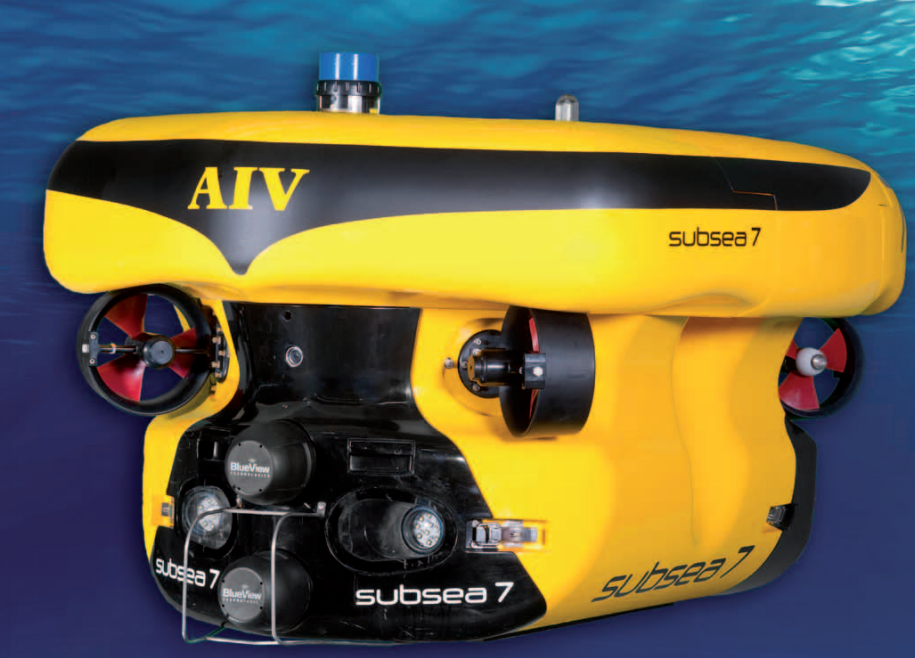
\includegraphics[width=0.48\textwidth]{subsea7AIV}
	\end{center}
	
	\caption{Subsea 7's AIV. This is the first commercial autonomous inspection vehicle for subsea operations \cite{pressAIV}}
	%\vspace{-20pt}
\end{wrapfigure}

Subsea maintenance is perhaps the field that have seen the greatest advancements in autonomous inspection and maintenance. As offshore installations are moved to the seabed, maintenance and inspection has become a significant challenge. This has resulted in a widespread use of \acp{ROV}. Recent developments in other fields, e.g. computer vision, human-robot collaboration and machine learning, has resulted in new \acp{AIV} and \acp{AUV} capable of performing inspection and simple maintenance tasks autonomously\cite{subseaAIV}\cite{Ridao2015227}. A driving factor behind the transition from \acp{ROV} to \acp{AUV} is cost reduction through increased offshore campaign efficiency.

\subsubsection{Disaster Responce}

\begin{wrapfigure}{r}{0.5\textwidth}
	%\vspace{-20pt}
	\begin{center}
		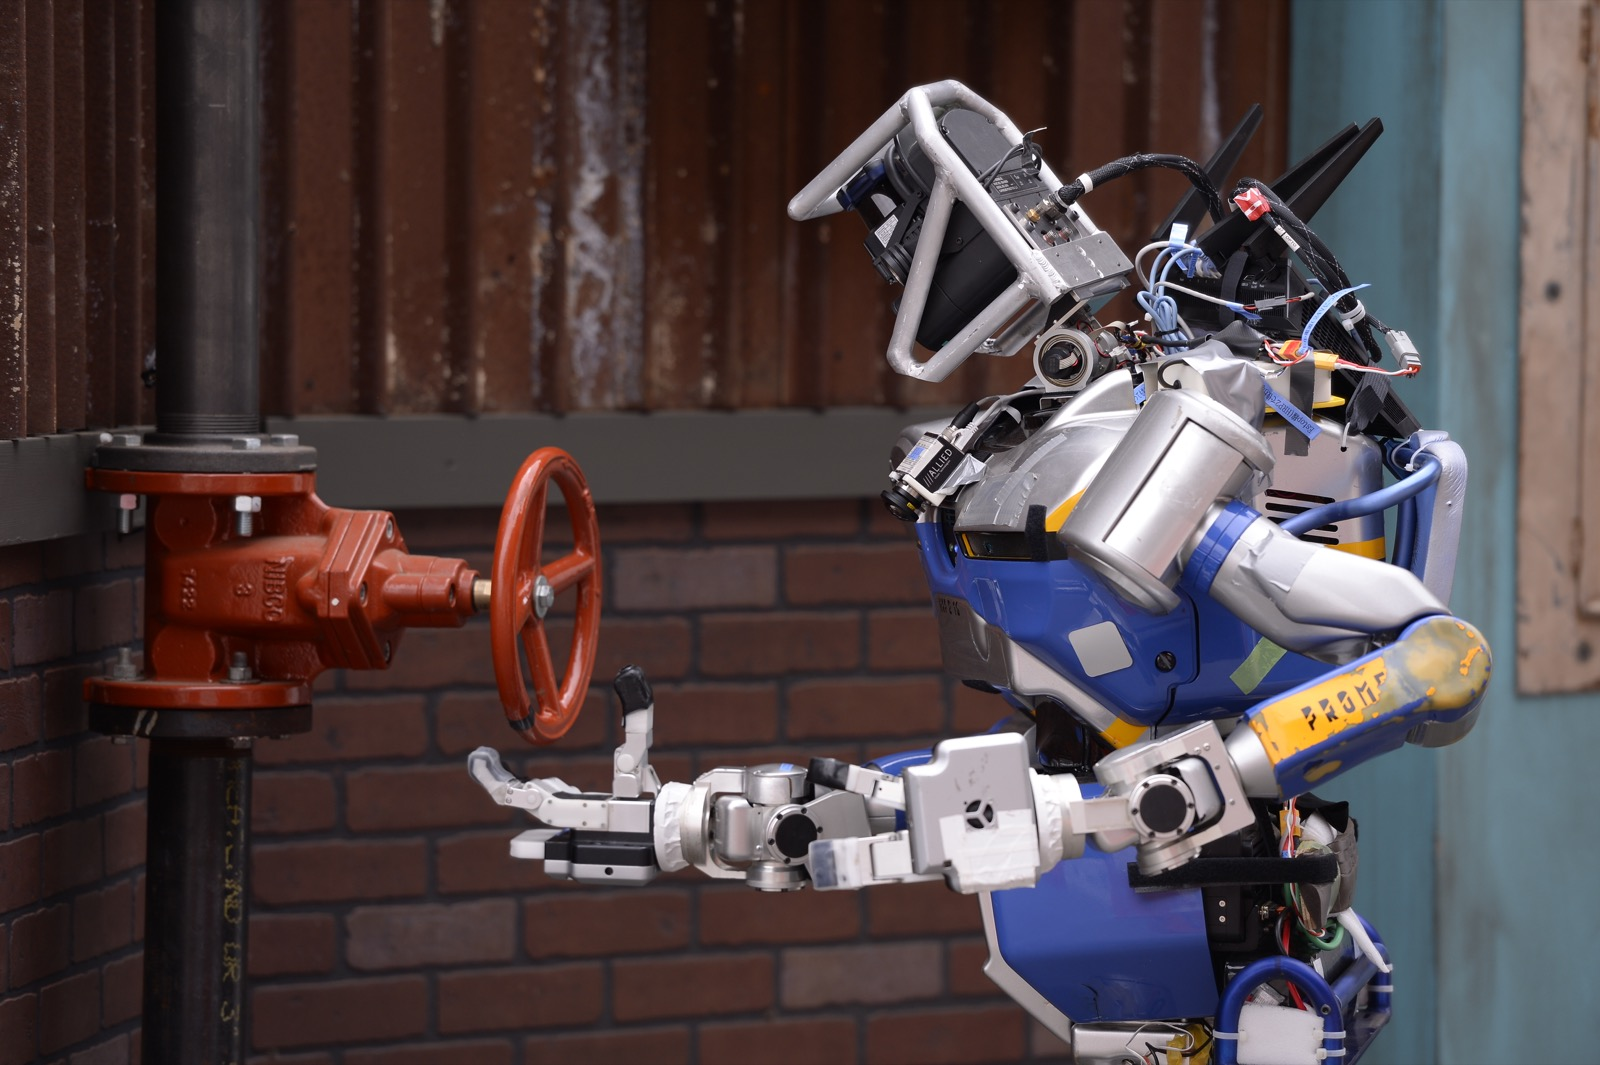
\includegraphics[width=0.48\textwidth]{HRP2_valve}
	\end{center}
	
	\caption{Team HRP2-Tokyo's robot turning a valve during DARPA Robotics Challenge 2015 (Image credits: DARPA Robotics Challenge)}
	%\vspace{-20pt}
\end{wrapfigure}

Robots in disaster response, relief and recovery solve many of the same problems faced by maintenance robots. Disasters, such as the tsunami which struck Japan in 2011, proved that much work needs to be done, both in terms of technical capabilities and logistical issues related to deployment and response times. The tsunami resulted in three core meltdowns at the Fukushima Daiichi Nuclear Power plant.

Many of the robots which were deployed at the Fukushima Power Plant were already ageing, and the operators had to receive training before deployment, thus increasing the response time\cite{doi:10.1108/01439911211249715}. A paper from Japan Atomic Energy Agency\cite{doi:10.1108/01439911211249715} highlights how the lack of stakeholder involvement could have been the cause of long response times. The same paper points out that the robots were developed for the sake of development, and not with emergency response as the main purpose\cite{doi:10.1108/01439911211249715}. 

\ac{DRC}\cite{DRC} was launched in response to the Fukushima disaster of 2011. The purpose of the competition is to accelerate innovation, research and development in robotics for disaster response in cases where humans cannot operate. Some of the tasks the competitors faces in 2015 include valve turning, traversing rubble and driving a vehicle through a course before egressing out of the vehicle.

\subsubsection{Topside Offshore and Onshore Robotic Maintenance}

Today, autonomous and teleoperated inspection and maintenance is usually only found at subsea installations. Topside installations on the other hand are still maintained and inspected manually, with some notable exceptions. Small \acp{UAV} or \acp{RPAS} have become commonplace over the last decade. On topside installations, they are being used for visual inspection of inaccessible structural parts such as flare stacks or the exterior of oil rigs.

\begin{wrapfigure}{l}{0.45\textwidth}
	%\vspace{-20pt}
	\begin{center}
		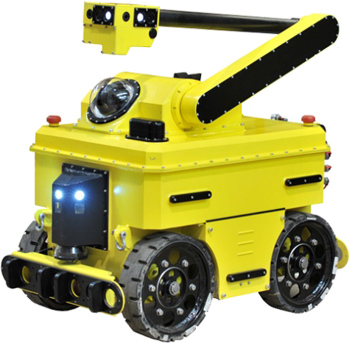
\includegraphics[width=0.42\textwidth]{sensabot}
	\end{center}
	
	\caption{An early version of the maintenance robot ''Sensabot'', developed by National Robotic Engineering Center (NREC) (Image credits: NREC)}
	%\vspace{-20pt}
\end{wrapfigure} 

Among the research groups working on robotic maintenance for \ac{OG}, ABB, \ac{Fraunhofer IPA} and NREC  at  Carnegie
Mellon University stand out as major contributors to the field. 

NRECs contribution, Sensabot, is a remotely operated inspection robot designed for harsh and remote environments\cite{deploymentsensabot}. It is not designed to be autonomous, but rather as a tool to move personnel from hazardous environments to safe remote control rooms. Sensabot mark II will be certified for zone 1 explosive environments. This year (2016), the plan is to test the robot on site at the Kashagan field in Kazakhstan\cite{peerless2016robot}.

\ac{Fraunhofer IPA}\footnote{http://www.ipa.fraunhofer.de/en.html} has developed a robot, called \ac{MIMROex}, with capabilities which are quite similar to the prototype used during the work on this thesis. \ac{MIMROex} is equipped with a camera for visual inspections as well as microphones, vibration and sensors for fire and gas detection. It is also certifiable in accordance with the explosion protection standard IEC 60079\cite{MIMROex}. 

Another effort towards robotic maintenance is the ARGOS challenge (Autonomous Robot for Gas and Oil Sites). The purpose of the challenge is to promote innovation, understanding and awareness towards robotic maintenance of \ac{OG} sites in harsh environments\cite{ARGOS}.

\section{Modelling and Simulation}

\subsection{Some Terminology}

\subsubsection{Coordinate Systems and Poses}

\subsubsection{Robot Joints}

All links are connected to each other by joints. 

Coordinate systems are essential in the field of robotics. 

\subsection{Robot Modelling}

\subsection{Simulating in Gazebo}

\section{ROS}

\subsection{Introduction}

The \ac{ROS} is a collection of software libraries, tools and drivers intended for robot software development. A \ac{ROS} installation can be tailored to meet the demands of a wide range of robots with varying complexity. \ac{ROS} is usually installed in the form of an already built Debian-package. These packages are only compatible with a few versions of Ubuntu which are specified on the \ac{ROS} homepage. When installed and configured, \ac{ROS} will run on top of Linux, and can be perceived as and extention of Linux itself. Installing \ac{ROS} from source is possible, but not recommended \cite{ROS_install}.

Roots of \ac{ROS} can be traced back to Stanford University at the beginning of the 2000s. At Stanford, several robotics software frameworks, including \ac{STAIR} and the \ac{PR} program, were created to provide dynamic, flexible and well tested foundations for further robot development and research. In 2007, a nearby start-up company and robot incubator, Willow Garage, sought to build upon these concepts, and initiated a collaborative and open development process of a new software framework. This framework eventually became \ac{ROS}\cite{ROS_history}\cite{rosbook15}. The framework can be used under the BSD open-source license\cite{BCD_license}. Today, \ac{ROS} comes in many forms and comprise hundreds of advanced packages, algorithms and drivers, making it applicable for hobbyists, industrial automation, research and everything in between. 

\subsection{Important ROS Concepts}

The following descriptions are included in order to provide a complete, self-contained description of the project implementation. Similar descriptions can be found on the official \ac{ROS} website\footnote{\url{http://www.ros.org/}}, as well as in any book on \ac{ROS} (for example \cite{rosbook15}). 

\subsubsection{The ROS Graph}

A \ac{ROS} system comprise a set of small programs that communicate with each other through messages. These programs become nodes in the \ac{ROS} graph. The nodes communicate with each other by publishing and subscribing to topics that form the edges of the graph. A topic must have the format of one of the specific data types provided by \ac{ROS}. For example, a node which receives temperature data from a thermometer, may publish the data as a topic on the \ac{ROS} system with the type \texttt{sensor\_msgs/Temperature}. There are many other data formats, e.g. velocity messages, \texttt{geometry\_msgs/Twist}; images, \texttt{sensor\_msgs/Image}; odometry messages, \texttt{nav\_msgs/Odometry} and so on. Each node in the graph are typically POSIX processes, and the edges are TCP connections\cite{rosbook15}. A minimal example of a graph is shown in figure \ref{fig:minimum_graph}.

\begin{figure}[p]
    \centering
    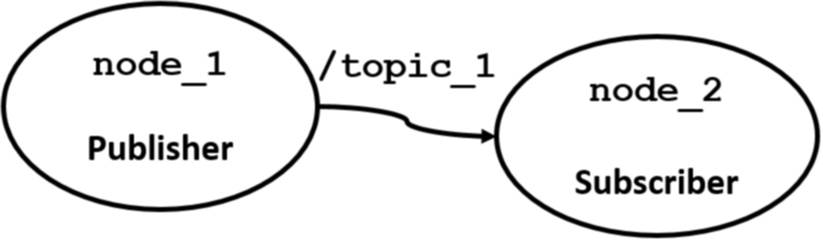
\includegraphics[width=0.8\textwidth]{minimum_graph_bl}
    \caption{A minimal \ac{ROS} graph. There are two nodes, none 1 and node 2. Node 1 publishes data, i.e. a topic, by the name \texttt{topic\_1}. Node 2 can receive the data by subscribing to \texttt{topic\_1}.}
    \label{fig:minimum_graph}
\end{figure}

\subsubsection{roscore}

\texttt{roscore} is an essensial part of any \ac{ROS} system as it enables nodes to communicate with each other. An instance of \texttt{roscore} must be started before launching any nodes. When a node is started, it will inform \texttt{roscore} of which topics it publishes and which topics it wish to subscribe to. Then, \texttt{roscore} will provide the information which allows the node to form a peer-to-peer connection to other nodes.

\subsubsection{Project Structure and the \textit{catkin} Build System}

The source code in a \ac{ROS} system is organized into packages. Each package provides a specific functionality to the system. Some packages can be downloaded and installed from a remote repository, while other packages will be created by the in-house developers for their specific robotic system. In this project, locally created ROS-packages were placed into a \textit{catkin workspace}. This workspace contains the  original source code and build specifications. Details are provided in chapter \ref{chp:implementation}. As presented in\cite{ROS_tut_pkg}, a general workspace structure is as follows:

\begin{verbatim}
workspace_folder/        -- CATKIN WORKSPACE
  src/                   -- SOURCE SPACE
    CMakeLists.txt       -- 'Toplevel' CMake file, provided by catkin
    package_1/
      CMakeLists.txt     -- CMakeLists.txt file for package_1
      package.xml        -- Package manifest for package_1
    ...
    package_n/
      CMakeLists.txt     -- CMakeLists.txt file for package_n
      package.xml        -- Package manifest for package_n
\end{verbatim}

A \ac{ROS} project will usually utilize the catkin build system.



\subsection{An Overview of ROS-Related Tools}

\subsubsection{Robot Modelling In URDF}

\ac{URDF} is an XML-like format for describing robots. The robot description is made up of links and joints. Each link description contains information of its shape, inertial tensor, collision boundaries. The links are connected to each other by joints.

\subsubsection{Visialization in \texttt{rviz}}

\texttt{rviz} is an invaluable tool for visualizing on-line robot behaviour. Simply put, \texttt{rviz} is created to visualize what the robot sees, and how it plans ahead. Many of the images in the following chapters are from \texttt{rviz}. 

\subsubsection{Simulation in Gazebo}


\subsection{Notable Robots Running ROS}

\paragraph{PR2 - Personal Robot 2}

PR2 is one of the first robots designed to run \ac{ROS} \cite{rosbook15}, and also one of the most advanced and capable robots with \ac{ROS} today. 

\paragraph{TurtleBot} 

TurtleBot is a cheaper ROS-ready alternative to PR2. 

\paragraph{Robonaut 2}

Robonaut 2, a dexterous humanoid robot, currently resides within the \ac{ISS} 400 km above the earth's surface. In 2014, a SpaceX Dracon capsule brought \ac{ROS} as well as a pair of legs for Robonaut up to the \ac{ISS}\cite{ROS_space}. Robonaut is designed for research on human-robot collaboration in space, and human-like tasks. For more information, follow \href{https://vimeo.com/106993914}{\textbf{this link}}\footnote{\url{https://vimeo.com/106993914}} to a talk on \ac{ROS} in space from ROSCon 2014.

Being the first robot with \ac{ROS} to be launched into space, 

\paragraph{Example of an industrial robot with ROS goes here!}

TODO!!!!!!!!!!

\section{Software}

\subsection{Qt}

\subsection{PCL}

\section{The Kinect Sensor}

\section{Software Tools}

\subsection{Point Cloud Library}

\subsection{ROS}

\subsection{Qt}


\subsection{Current Research and Applications}

\section{Introduction to Sensors in Autonomous Robots}

\subsection{Depth Cameras}

\subsubsection{Different Methods for Depth Perception}

A depth camera can be described as a regular color video camera with the ability to create spatial images. In the context of this thesis, a depth camera can  more precisely be described as a RGB-D camera, where the letters RGB-D are short for red, green, blue and depth. In a regular RGB camera, a spatial scene will be projected onto a rectangular pixel grid where each pixel contains intensity values for red, green and blue colors. These pixel values represents the detected scene. A major problem with RGB cameras is the significant loss of information. The information loss is mostly a consequence of 3d to 2d projection and digital quantization. RGB-D cameras have the means to reduce this information loss by mapping the pixel values to spatial coordinates. The atomic parts in 3d images are usually represented as point clouds or cubic volumes, also known as voxels.

Different variations of depth cameras will usually fall into one of two categories: active or passive. Passive sensors perceive the surroundings as it is, without actively interfering with the environment as a part of the sensing process. A typical passive RGB-D sensor is the stereo camera. Stereo cameras use a stream of synchronized image pairs to perceive depth. The image pairs are displaced along the horizontal axis, and the depth information is extracted by searching for mutual information in the image pairs. How far the information is displaced from the left to the right image is directly related to how far away from the camera the information source is located. 

Active sensors depend on some form of projection onto the surroundings. For depth cameras, the projection is usually in the form of laser or infra red light. In RGB-D cameras it is essential that the projected light is distinguishable from the visible spectrum. The Kinect sensor used in this project is an example of an active RGB-D sensor. A proper introduction to the Kinect, will follow shortly.

\subsubsection{Natural User Interfaces - Origin of the Kinect}

The idea behind a \ac{NUI} is to make \ac{HMI} as seamless and natural as possible. A \ac{NUI} allows the user to communicate without tools such as a keyboard or a mouse. For decades, \ac{NUI}s have only existed as ideas, science fiction or research projects. This has changed dramatically over the last ten years, and \ac{NUI}s can now be considered to be ubiquitous. Today, the most common form of \ac{NUI}s is the touch screen found in smart phones and tablets. 

The Microsoft Kinect sensor was initially designed as a \ac{NUI} for the Xbox 360 gaming console. The sensor allows users to use gestures and sounds to play console games. Later on, Microsoft has released SDKs, enabling developers to create \ac{NUI} applications for for Windows. 

\subsubsection{Kinect for Xbox 360}

Kinect for Xbox 360 is the RGB-D sensor used in this project. The device  was initially intended as a \ac{NUI} for gaming and office applications, and was the first consumer grade sensor to utilize structured light. Possible use cases were inspired by early \ac{NUI} research at \ac{MIT} and, later on, the science fiction movie Minority Report, where Tom Cruice interacts with a computer by using hand gestures \cite{kinect_book}. The Kinect sensor is equipped with a depth sensor, a regular color camera, a microphone array and a tilt motor. The color camera in combination with the depth sensor forms what is usually referred to as a RGB-D sensor, i.e. a combined color and depth camera (figure \ref{fig:kinect360_exp}). This feature, combined with the relaticely low cost and accessability of the sensor has contributed to make the Kinect very popular in research projects related to \ac{SLAM} and robotics. In the three first years since it's release in 2010, over 3000 papers in well-known journals and proceedings were devoted to research on the Kinect sensor. Roughly 500 of these papers focused on \ac{SLAM} or 3d reconstruction\cite{Berger2013}. Some of the other papers focused on some of the weaknesses with the sensor, such as detection of glass surfaces and having several sensors in the same area. 


Today, the the Kinect for Xbox 360 has been succeded by the Kinect for Xbox One, and is now considered to be a legacy device. Those considering to use the legacy Kinect should be aware of that it is becoming increasingly difficult, if not already impossible, to get hold of a new Kinect for Xbox 360. 

\begin{figure}[p]
    \centering
    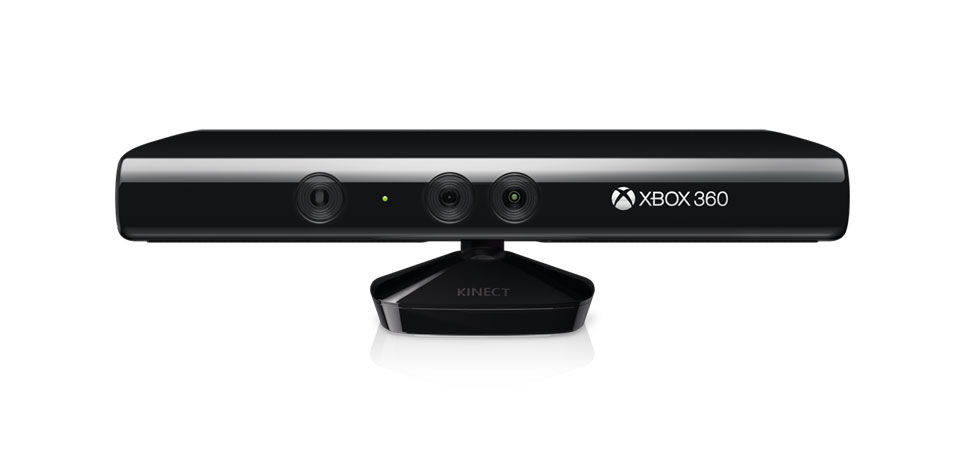
\includegraphics[width=0.8\textwidth]{kinect360}
    \caption{Awesome Image}
    \label{fig:kinect360}
\end{figure}

\begin{figure}[p]
    \centering
    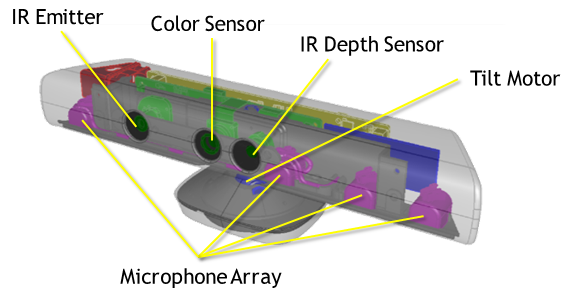
\includegraphics[width=0.8\textwidth]{kinect360_exp}
    \caption{Awesome Image}
    \label{fig:kinect360_exp}
\end{figure}


\subsection{Plannar Laser Sensors (LIDAR)}

A plannar laser sensor, known as e.g. laser proximity sensors or laser radars, can all be referred to as LIDARs. 

\subsubsection{Scanning Laser Range Finder, URG-04LX-UG01}


\subsection{Odometers}

\subsection{Sensor Fusion}


\section{Simultanious Localization and Mapping (SLAM)}

\subsection{Introdunction to SLAM}

\ac{SLAM}, also known as \ac{CLM}, is a class of solutions to the problem of determining an agents location and pose in an unknown environment, while simultaneously mapping the same environment.

\subsection{Hector SLAM}

\subsection{RTAB-Map}

\ac{RTAB-Map} is developed by IntRoLab at Université de Sherbrooke in Canada. It is a \ac{SLAM} system developed for long term operations in large environments. The system is also intended to handle the ''kidnapped robot-problem'', i.e. multi-session mapping. This is useful whenever the robot is shut down and moved to an unmapped part of the same area, where it will start a new mapping session. \ac{RTAB-Map} is the core feature that has been integrated into the robot described in this thesis. Some factors which motivated the use of \ac{RTAB-Map} are:

\begin{itemize}
	\item It is a \ac{SLAM} method which requires an RGB-D sensor, for example a Kinect. The problem description for this project requires a vision based solution.
	\item \ac{RTAB-Map} has a \ac{ROS} wrapper, \texttt{rtabmap\_ros}, which eases the process of integrating it with the mobile robot.
	\item It includes 3d obstacle detection.
	\item It has a memory management system intended for large scale multi-session mapping.
	\item \ac{RTAB-Map} can be used for object detection. This can be done by linking \ac{RTAB-Map} to OpenCV and the non-free feature detectors \ac{SIFT} and \ac{SURF}.
\end{itemize}

The source code and \ac{ROS} wrapper is currently maintained, and new features and bug-fixes are added regularly. \ac{RTAB-Map} has two distinctive solutions to the \ac{SLAM} problem: Visual loop closure detection and a memory management system for large data sets. The following paragraphs provides an overview of how \ac{RTAB-Map} works. Detailed descriptions of the loop closure detection and memory management approach is provided in  \cite{labbe13appearance}, while the \ac{SLAM} method is presented in \cite{labbe14online}. Further details can be found on the project's Github page\footnote{\url{http://introlab.github.io/rtabmap/}}.

\subsubsection{Graph Based Mapping}

\ac{RTAB-Map} uses a graph structure with nodes and edges to represent the map. New nodes are continuously added to the systems working memory as time passes. In this method, the graph edges are referred to as \textit{links}. There are two types of links: neighbour links and loop closure links. Each node is a location in the map, and the links contain geometrical transformations between the node locations. Figure \ref{fig:rtabmap_graph} illustrated the graph concept.

\begin{figure}[p]
    \centering
    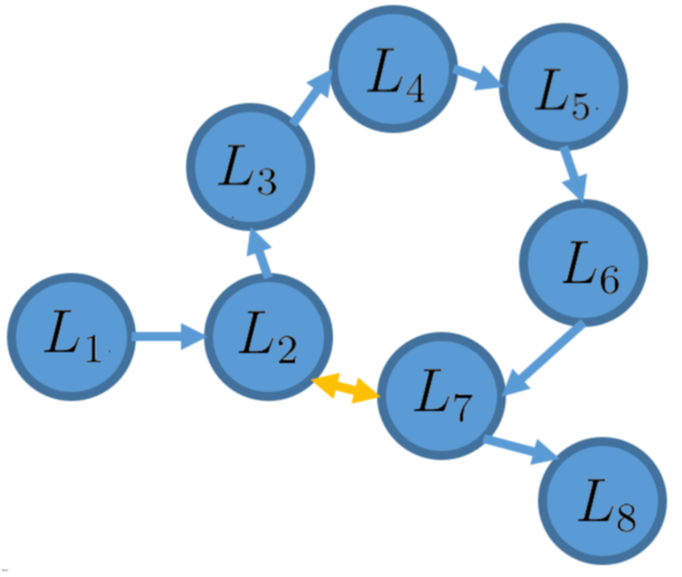
\includegraphics[width=0.5\textwidth]{rtabmap_graph_bl}
    \caption{Conceptual illustration of a graph created by \ac{RTAB-Map} over time $1 \leq t \leq 8 $. A loop closure hypothesis was accepted at $t=7$, as shown by the yellow arrow. Feature descriptors in $L_2$ and $L_7$ are sufficiently similar to accept this as a loop closure.}
    \label{fig:rtabmap_graph}
\end{figure}

\subsubsection{On-line Mapping of Large Environments}



\subsection{Octomap}

\section{Navigation}

\chapter{Implementation}
\label{chp:implementation} 

Implementation procedure for mobile robot:

\begin{itemize}

	\item Decide on ROS message interface.
	\item Write interfaces for the motor drivers.
	\item Create a description of the physical structure and properties of the robot in \ac{URDF}. 
	\item Extend the model to enable simulation in Gazebo.
	\item Publish coordinate transform data via \textit{tf} and visualize it in rviz.
	\item Add sensors, with driver and simulation support.
	\item Apply algorithms for navigation and other functionality. 

\end{itemize}

\section{Modeling}

\subsection{Physical Dimensions}

The inertia tensor:

\begin{equation}
    	I = \begin{bmatrix}
    	I_{xx} & I_{xy} & I_{xz} \\[0.3em]
    	I_{yx} & I_{yy} & I_{yz} \\[0.3em]
    	I_{zx} & I_{zy} & I_{zz}
    	\end{bmatrix}
\end{equation}

Inertia tensor for a solid, uniform cylinder where the radius $r$ is measured in parallel to the $x - y$ plane, and $h$ is parallel to the $z$ axis:
\begin{equation}
I_{cylinder} = \frac{1}{12}m \begin{bmatrix}
	(3 r^2 + h^2) & 0 & 0 \\[0.3em]
	0 & (3 r^2 + h^2) & 0 \\[0.3em]
	0 & 0 & r^2
	\end{bmatrix}
\end{equation}

Inertia tensor for a solid, uniform cuboid. The subscript of $l$ indicates which axis $l$ is measured along:
\begin{equation}
I_{cuboid} = \frac{1}{12}m \begin{bmatrix}
	(l_y^2 + l_z^2) & 0 & 0 \\[0.3em]
	0 & (l_x^2 + l_z^2) & 0 \\[0.3em]
	0 & 0 & (l_x^2 + l_y^2)
\end{bmatrix}
\end{equation}

\subsection{Coordinate Frames}

\section{Simulations}

\section{ROS Nodes for Motion Control}


\subsection{Velocity Command Sources}

There are four ways to control the robot:

\begin{itemize}
	\item Local keyboard input.
	\item Wireless teleoperation from the \ac{OCS}.
	\item Wireless teleoperation from a handheld Bluetooth device.
	\item Commands from the navigation stack in \ac{ROS}.
\end{itemize}

\begin{figure}[p]
	\centering
	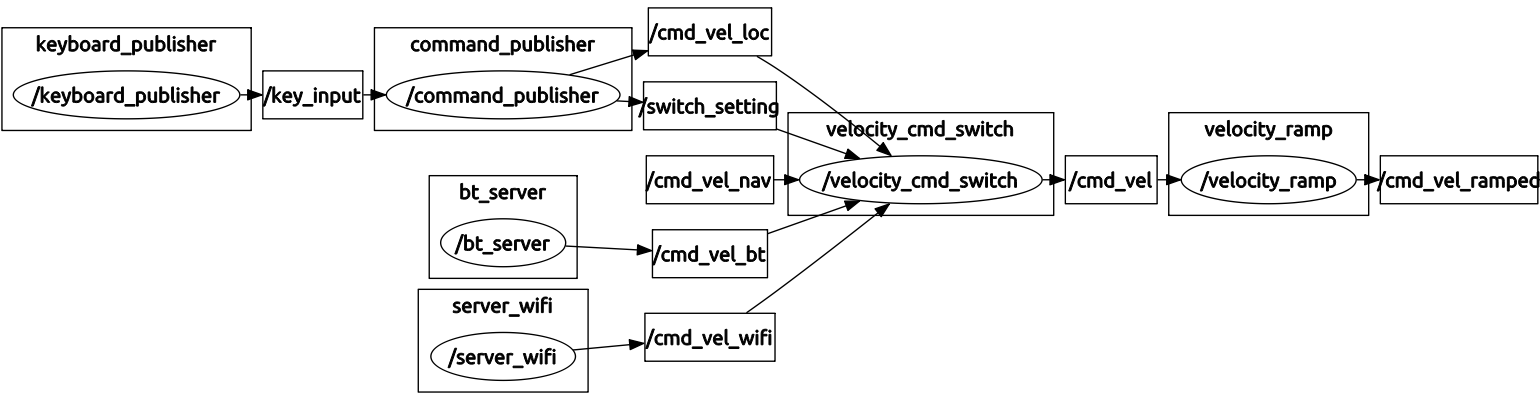
\includegraphics[width=1\textwidth]{move_base_nodes}
	\caption{Nodes and topics for motion control. }
	\label{fig:move_base_nodes}
\end{figure}

\begin{figure}[p]
	\centering
	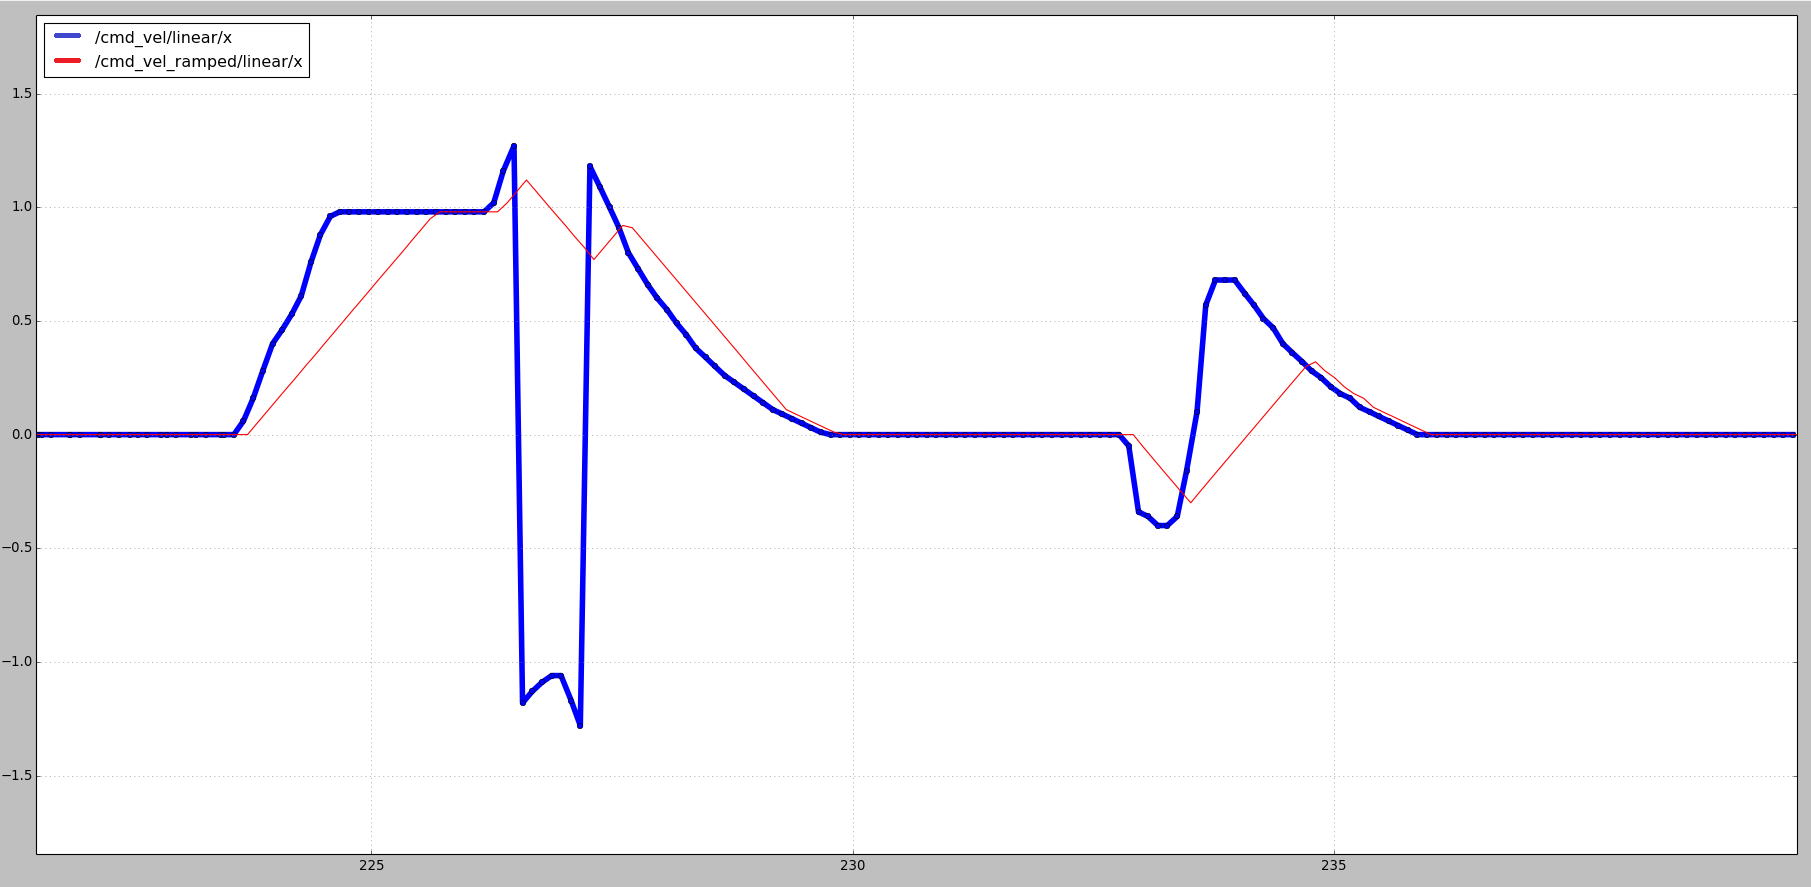
\includegraphics[width=1\textwidth]{velocity_ramp_cropped}
	\caption{Velocity command ramping. The blue line represents commands entering \texttt{''velocity\_ramp''}, while the red line shows the acceleration constrained output command.}
	\label{fig:velocity_ramp}
\end{figure}

\section{Operator Control Station (OCS)}

The \ac{OCS} allows an operator to control and monitor the robot through a graphical user interface. \texttt{MainWindow}

\subsection{Graphical User Interface}

A Qt-based \ac{GUI}...

\section{The Handheld Remote Control - "Robot Leash"}

Because the \ac{OCS} is only partially implemented, an operator will not have access to all the features on the robot. In addition, as a safety precaution a person should be close to the robot at all times, and be ready to pull the plug. Furthermore, it is hard to control a moving robot through the on-board keyboard. These problems were countered by the Android-based remote control, ''Robot Leash''. 


\begin{figure}
	\centering
	\begin{subfigure}[b]{0.30\textwidth}
		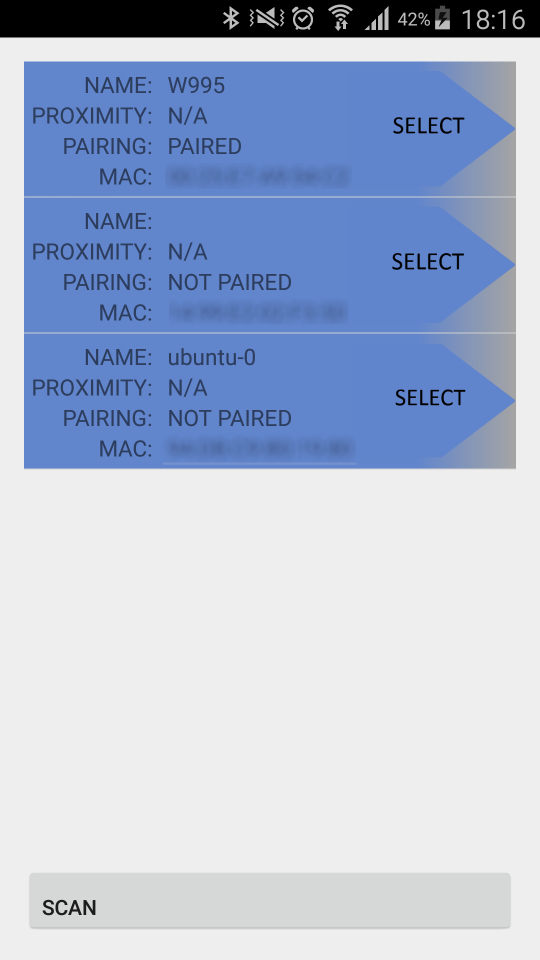
\includegraphics[width=\textwidth]{device_select}
		\caption{First activity with device list.}
		\label{fig:device_select}
	\end{subfigure}
		\begin{subfigure}[b]{0.30\textwidth}
			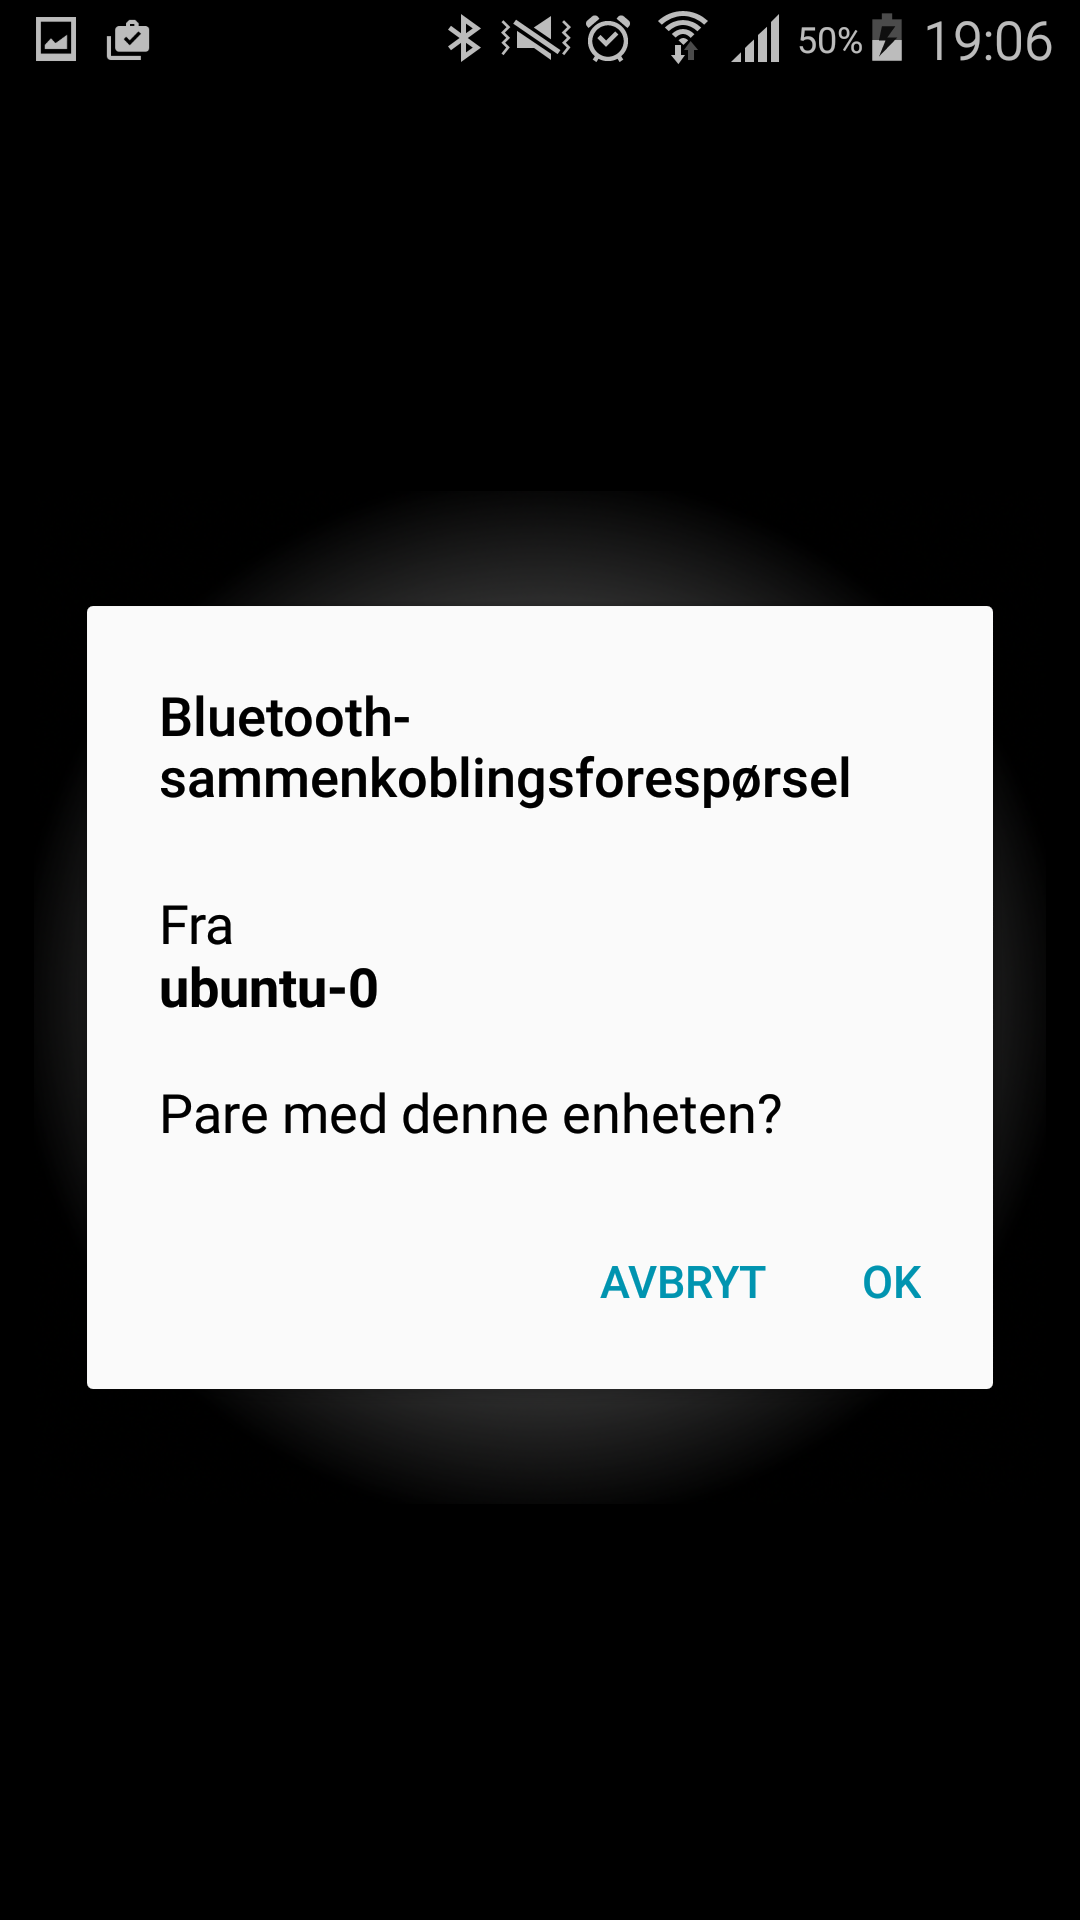
\includegraphics[width=\textwidth]{bt_request}
			\caption{The user is prompted to pair with the robot.}
			\label{fig:bt_request}
		\end{subfigure}
	\begin{subfigure}[b]{0.30\textwidth}
		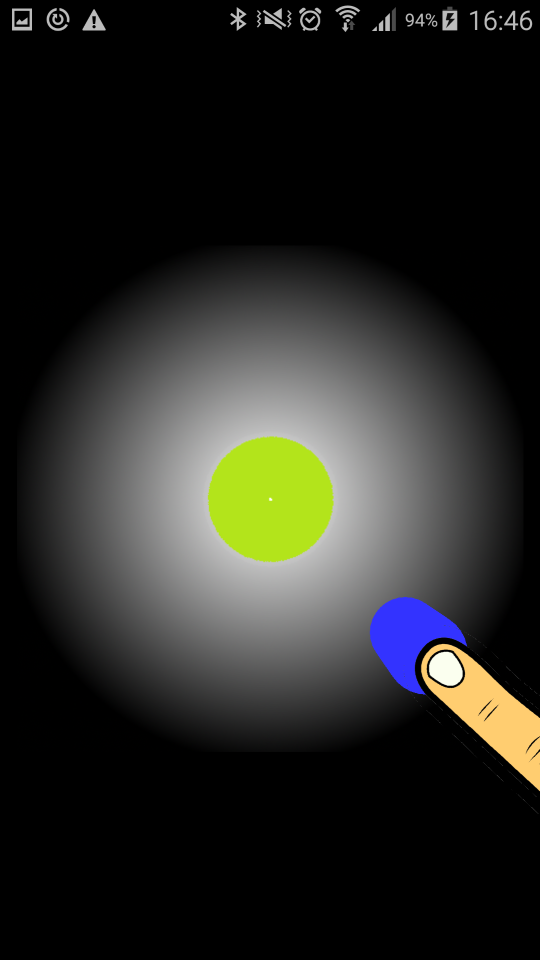
\includegraphics[width=\textwidth]{using_app}
		\caption{Controlling the robot with the stick.}
		\label{fig:using_app}
	\end{subfigure}
	\caption{\label{fig:app_screens}A typical use case for ''Robot Leash''.}
\end{figure}

\subsection{Connecting to a the Robot}

\begin{enumerate}
	\item The first screen after scanning for devices. There is no device filtering, and the user can select any device, but only connect through a specific service.
	\item After selecting a device which provides the correct service, the user will be prompted to pair the devices.
	\item The smartphone and the robot is now paired, and velocity commands from the blue control stick are passed to the robot via Bluetooth.
\end{enumerate}

http://developer.samsung.com/technical-doc/view.do?v=T000000117

\chapter{Results}
\label{chp:results} 

\section{Introduction}

This chapter presents how the robot and the supporting implementations were tested and the results that where obtained. The same software system was used for both the simulated and live robot. It was still necessary to have some separate launch and configuration files for the simulated and hardware version (section \ref{sec:integration}). Section \ref{sec:testplan} provides an overview of the various features and components which were tested, and how these items are assessed. Next, in section \ref{sec:results_summary}, a brief overview of the results are presented. The two last sections will go through the more nuanced results and events from the simulations and live trials respectively. It was difficult to come up with a rigorous test plan because of time constraints. Much of the testing was done together with parameter tuning. 


\section{Testplan}
\label{sec:testplan}
The tests listed in tables \ref{tab:support_func} and \ref{tab:main_func} will be carried out in the simulator, as well as in the real world. They will mainly focus on the navigation stack and \ac{RTAB-Map}. 

\begin{table}
	\centering
	\begin{tabular}{ p{3.5cm} | p{7cm} }
		\multicolumn{2}{c}{Supporting Functionality}\\
		\hline
		\textbf{Evaluate} & Description\\
		\hline
		\textbf{Mobile application, ''Robot Leash''} & Use the mobile application to manually steer the robot.\\
		\hline
		\textbf{Operator Control Station} & Steer the robot from the \ac{OCS} while monitoring the robot through the live video stream. \\
		\hline
		\textbf{Motor controller on XMEGA A3BU} & Verify ability to command the wheels. Confirm that the vehicle stops when velocity commands from \ac{ROS} are absent.\\
		\hline
	\end{tabular}
	\caption{Supporting Functionality}\label{tab:support_func}
\end{table}

\begin{table}
	\centering
	\begin{tabular}{ p{2.5cm} | p{7cm} }
	\multicolumn{2}{c}{Core Functionality}\\
\hline
	\textbf{Evaluate} & Description\\
	\hline
	\textbf{Multi Session Mapping} & Verify that the robot can rediscover areas which have been mapped in a previous mapping session.\\
	\hline
	\textbf{Loop Closure Detection} & As a core functionality in \ac{RTAB-Map}, it is critical to evaluate the loop closure mechanism.\\
	\hline
	\textbf{Autonomous Navigation} & Perform a set of tests on the navigation stack. The tests should evaluate path planning with moving obstacles. Different parameters should be tested and evaluated. Observe how the robot handles narrow passages. Evaluate robustness of the navigation stack for this robot.\\
	\hline
	%\caption{}
	\end{tabular}
	\caption{Core Functionality}\label{tab:main_func}
\end{table}

\section{Brief Summary of All Results}
\label{sec:results_summary}
%\begin{table}
%	\centering
%	\begin{tabular}{ p{3.5cm} | p{7cm} }
%		\multicolumn{2}{c}{Result Summary}\\
%		\hline
%		\textbf{Test Item} & Evaluation\\
%		\hline
%		\textbf{Mobile application, ''Robot Leash''} & The mobile App works as expected. The user can connect to the robot and send velocity commands to the real and simulated mobile base via Bluetooth. This tool proved to be invaluable, and was used during all mapping sessions.\\
%		\hline
%		\textbf{Multi Session Mapping} & An example of multi session mapping was recorded to the video \texttt{live\_multi\_session\_mapping} enclosed in the DVD. The live robot can successfully merge multiple maps. In Gazebo, the method is more vulnerable to similar features in different parts of the world.\\
%		\hline
%		\textbf{Loop Closure Detection} & Successful live loop closure detection is demonstrated in the video \texttt{live\_mapping\_succesful}. The simulated environment was a bit more challenging, as demonstrated in the enclosed video \texttt{sim\_wrong\_loop\_closure}.\\
%		\hline
%		\textbf{Autonomous Navigation} & Autonomous navigation was evaluated based on the ability to reach a feasable goal state, and the ability to avoid static and dynamic obstacles. The global planner works as expected in both the simulator and in the real world. The simulated robot was frequently unable to reach its goal. The real robot successfully navigated a static and dynamic obstacle course (video \texttt{live\_navigation\_1} and \texttt{2}, and ''Obstruction detection and avoidance'').\\
%		\hline
		%\caption{}
%	\end{tabular}
%	\caption{Result Summary}\label{tab:result}
%\end{table}

\subsubsection{Mobile application, ''Robot Leash''}

The mobile App works as expected. The user can establish a Bluetooth connection to the robot and send velocity commands to the real and simulated mobile base. This tool proved to be invaluable, and was used during all mapping sessions, both real and simulated.

\subsubsection{Operator Control Station}

\subsubsection{Motor controller on XMEGA A3BU}

An example of multi session mapping was recorded to the video ''\texttt{live\_multi\_session\_mapping}'' enclosed in the DVD. The live robot can successfully merge multiple maps. In Gazebo, the method is more vulnerable to similar features in different parts of the world.

\subsubsection{Loop Closure Detection}

Successful live loop closure detection is demonstrated in the video ''\texttt{live\_mapping\_succesful}''. The simulated environment was a bit more challenging, as demonstrated in the enclosed video ''\texttt{sim\_wrong\_loop\_closure}''.

\subsubsection{Autonomous Navigation}

Autonomous navigation was evaluated based on the ability to reach a feasable goal state, and the ability to avoid static and dynamic obstacles. The global planner works as expected in both the simulator and in the real world. The simulated robot was frequently unable to reach its goal. The real robot successfully navigated a static and dynamic obstacle course (video ''\texttt{live\_navigation\_1}'' and \texttt{2}, and ''Obstruction detection and avoidance'').



\section{Simulation Results}

The system was tested on a simulated model of the robot in Gazebo. A simulated environment, \texttt{Asphalt.world} shown in figure \ref{fig:gazebo2_cropped}, was populated with objects and clutter in order to provide a test environment with distinctive visual features for the visual mapping approach, and obstacles for the navigation stack. 
%An included simulator world of the Willow Garage office building was considered as a testing area. Unfortunately, the gray hallways and offices did not provide enough good visual features for \ac{RTAB-Map}.

\begin{figure}[h]
	\centering
	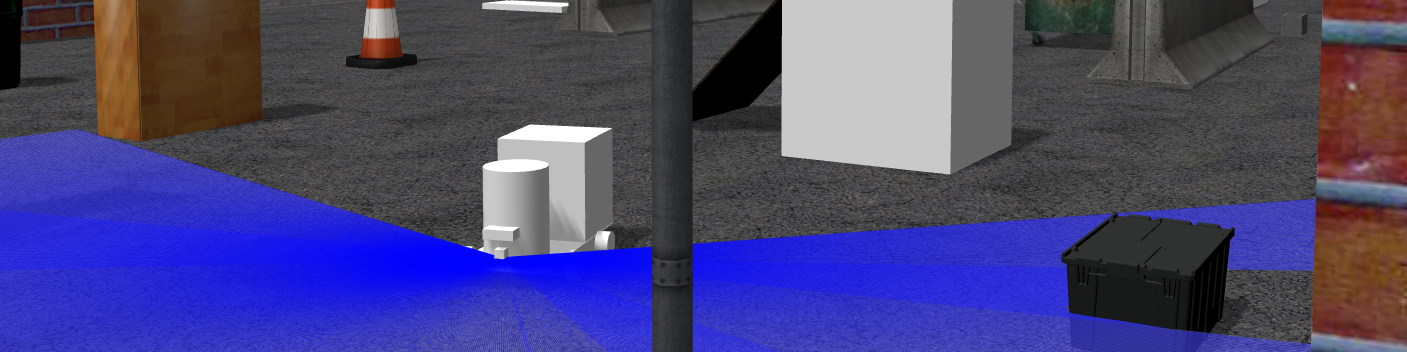
\includegraphics[width=1\textwidth]{gazebo2_cropped}
	\caption{The ''Asphalt'' world in Gazebo. }
	\label{fig:gazebo2_cropped}
\end{figure}

\subsection{Mapping}

\ac{RTAB-Map} on the robot in Gazebo allowed controlled testing of edge cases in a controlled environment. The ''Asphalt'' world proved to be a challenge for \ac{RTAB-Map} - at least with the parameters that were used during testing. Figure \ref{fig:rviz_mapping_trial} shows an example of a resulting 3D map. 

\begin{figure}[h]
	\centering
	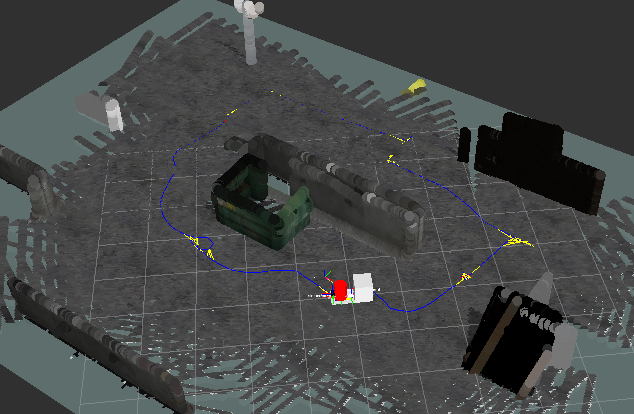
\includegraphics[width=0.7\textwidth]{rviz_mapping_trial_cropped}
	\caption{An example of a resulting point cloud map after running \ac{RTAB-Map} in Gazebo. }
	\label{fig:rviz_mapping_trial}
\end{figure}

The map quality varied greatly between the mapping trials. The path of the robot was found to have a significant impact on the recorded path between the stored locations in the \ac{RTAB-Map} system. An example of a problematic path is to drive the robot in parallel to a wall. Such a path creates few or none distinctive features as long as the robot follows this path. Figure \ref{fig:gazebo_lc_features} shows two problematic events. First, a loop closure is detected based on similarities detected on the asphalt plane. Because the loop closure is wrong, a wrong pose transform correction will be propagated backwards along the path of the robot, ultimately resulting in a displaced map.

\begin{figure}[h]
	\centering
	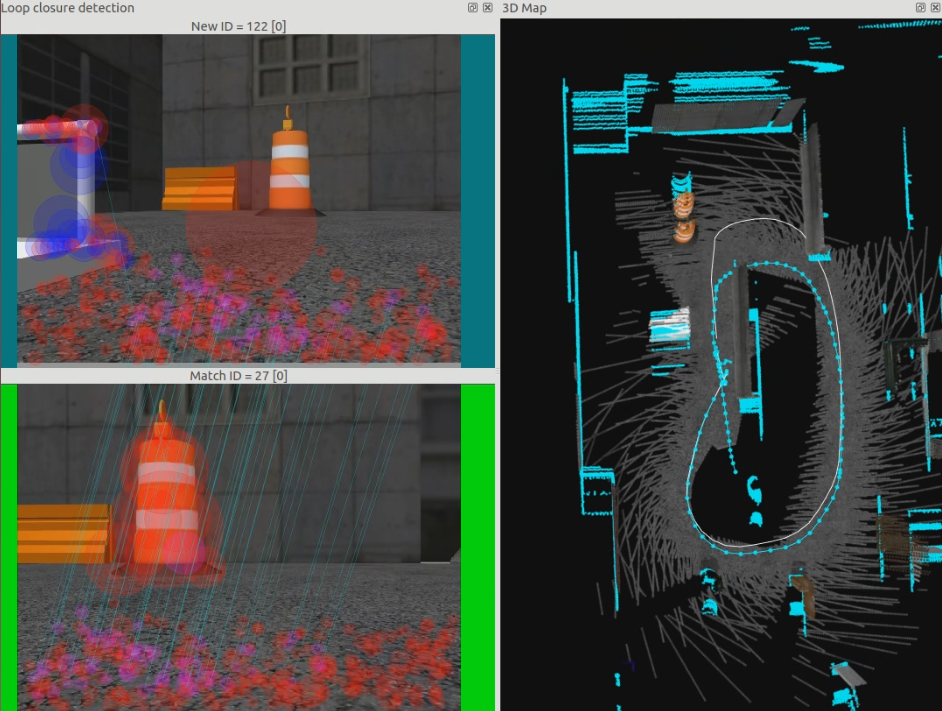
\includegraphics[width=0.9\textwidth]{gazebo_lc_features}
	\caption{Example of an incorrect loop closure detection. The pink circles indicate matching features. The right part shows an incorrect map adjustment. Observe how the matching features are located on the asphalt plane.}
	\label{fig:gazebo_lc_features}
\end{figure}

\begin{figure}[h]
	\centering
	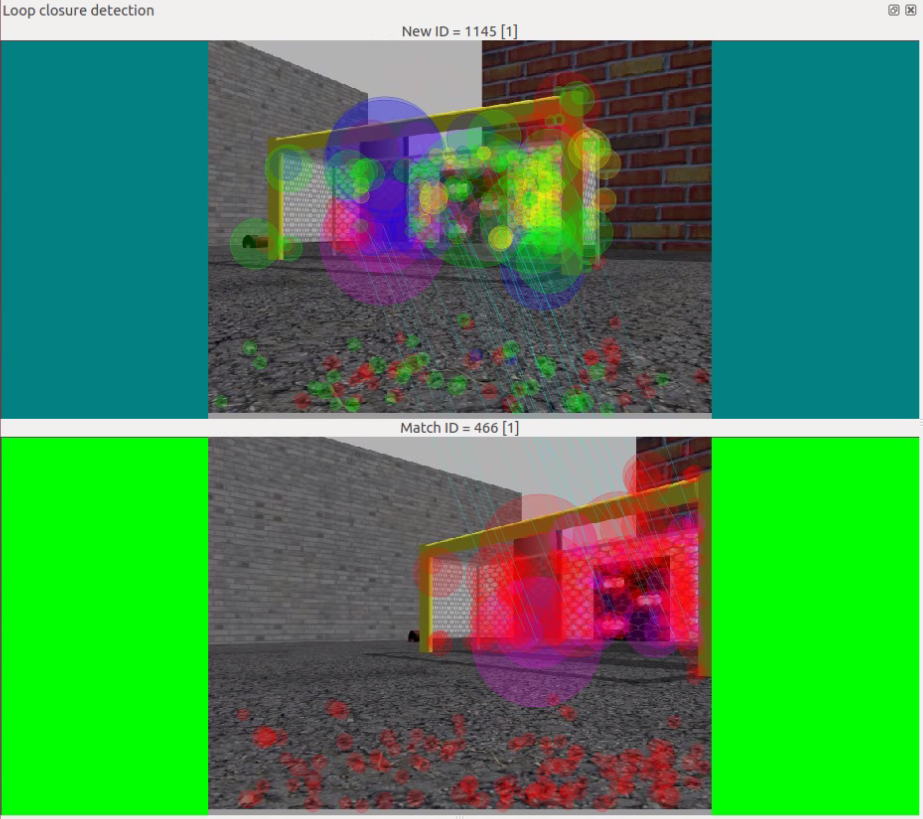
\includegraphics[width=0.9\textwidth]{loop_closure_detection}
	\caption{An example of an accepted and correct loop closure hypothesis. This example is from the ''Asphalt'' world simulated in Gazebo.}
	\label{fig:loop_closure_detection}
\end{figure}

Another error occurred during a multi session mapping trial. The robot detected a wrong loop closure at a location with similar features to a previously mapped location. This resulted in the map seen in figure \ref{fig:Incorrect_lc_detection}. Other localization problems were apparent when driving in open areas. The estimated location of the robot would fluctuate when turning the robot as features passed in or out of view.

Sensor settings is another factor that had a high impact on the \ac{SLAM} quality. When sensor ranges of the Gazebo sensor plugins are set according to the sensors technical specifications, both localization and mapping will struggle. An increased sensor range in for the simulated sensors would increase the \ac{SLAM} robustness.

\begin{figure}[h]
	\centering
	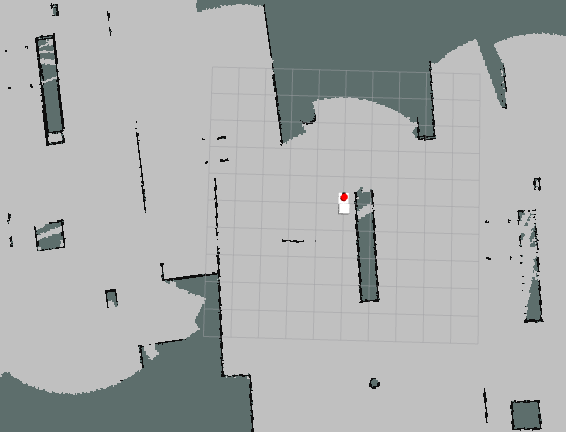
\includegraphics[width=0.75\textwidth]{Incorrect_lc_detection_cropped}
	\caption{An example of incorrect map merging. This case occurred in the ''Asphalt'' world simulated in Gazebo.}
	\label{fig:Incorrect_lc_detection}
\end{figure}


\subsection{Autonomous Navigation}

Testing the navigation stack in Gazebo fulfilled two goals. The first goal was to learn how the system behaved with different parameters and to uncover potential problems with the system before attempting to test the live robot. The second goal was to evaluate the ability to relocate the robot and avoid obstacles. 

The for the first trial, the robot footprint was extended well beyond the physical mobile base. The purpose of this was to prevent obstacles from getting too close to the Kinect and \ac{LIDAR}. As the minimum detectable range for the Kinect is $0.5 m$ (measured minimum depth), the footprint was extended $0.5 m$ beyond the front of the mobile base. A second parameter to be tuned is the obstacle inflation radius, i.e. the radius beyond each obstacle that is expensive or impossible to traverse. Figure \ref{fig:big_footprint} illustrates both the big footprint and the obstacle inflation radius.

During trials with the big footprint, the robot showed good collision avoidance capabilities but an aversion to narrow passages. Setting the obstacle inflation radius is also a dilemma in choosing between large margins for the global path or the ability to navigate through narrow passages. 

\begin{figure}[h]
	\centering
	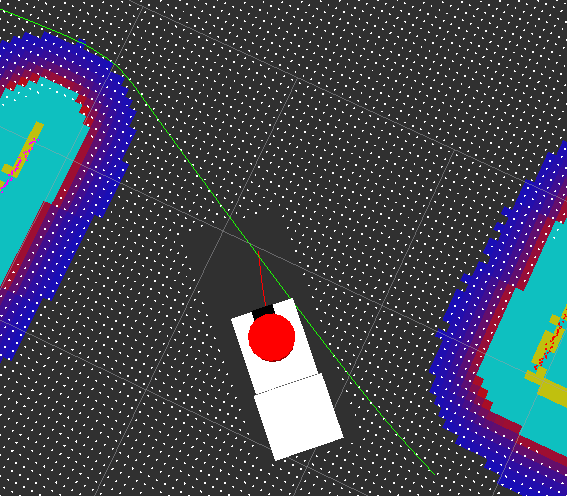
\includegraphics[width=0.7\textwidth]{planning_big_footprint_cropped}
	\caption{The robot footprint is illustrated by the clear rectangle that surrounds the robot model. The coloured areas are map locations with high cost. }
	\label{fig:big_footprint}
\end{figure}

In later navigation sessions, the robot footprint was reduced to a size slightly larger than the physical robot base. During some of the testing sessions, the robot would get stuck near obstacles. 

Sometimes, the robot would never actually reach the goal state, but rather circle around it. This problem was not solved, but more relaxed goal tolerances mitigated the issue a little. 

\section{Live Robot Results}

Due to time constraints, it was no time to tune the parameters of \ac{RTAB-Map}. \ac{RTAB-Map} is therefore used with the default parameters. An important distinction between the real and simulated system is found in the actuator, i.e. the motor controller of the mobile base. In the simulated system, the motor control card is emulated by a skid steering plugin. While the exact functionality of the skid steering plugin is unknown, it does ensure that the wheels follow the linear and angular velocity commands provided by \ac{ROS}. This is not the case for the real motor control card, as it lacks a feedback loop. The real robot velocity was in general slower that its simulated version.

\subsubsection{Safety Features}

The simulator offered the benefit of a risk free environment. This is not the case for the real robot. 

\subsubsection{Loop Closure Detection}

Loop closure detection was carried out on the first floor of Gamle Elektro at Gløshaugen, NTNU (figure \ref{fig:mapping_gamle_elektro}). This environment provides a good mix of featureless and feature rich surroundings. It will also provide an additional challenge because of the many students that use the hallways. Most importantly, there are loops in the environment that allow testing of vision based loop closures and odometry error correction. 

The first test run revealed two problems with the implementation, the first being odometry errors and the second being a failure to visually detect loop closures. Odometry based on laser scans would wrongfully indicate a change in the robot heading in some cases, and in other cases fail to correctly indicate heading changes when rounding corners. 

In later experiments it was found that different mapping techniques and path choices could either prevent or cause odometry errors. It was also found that it is helpful to start a mapping session in an area that is rich in distinctive features. The map and floor plan comparison shown in figure \ref{fig:comparison} shows a map where a loop closure was successfully detected. In the same figure, notice how the upper hallway is misaligned to the rest of the map. The robot failed to detect any good visual features in this area. Figure \ref{fig:lc_match_live} shows the resulting point cloud map of the same area.

\begin{figure}
	\centering
	\begin{subfigure}[b]{1\textwidth}
		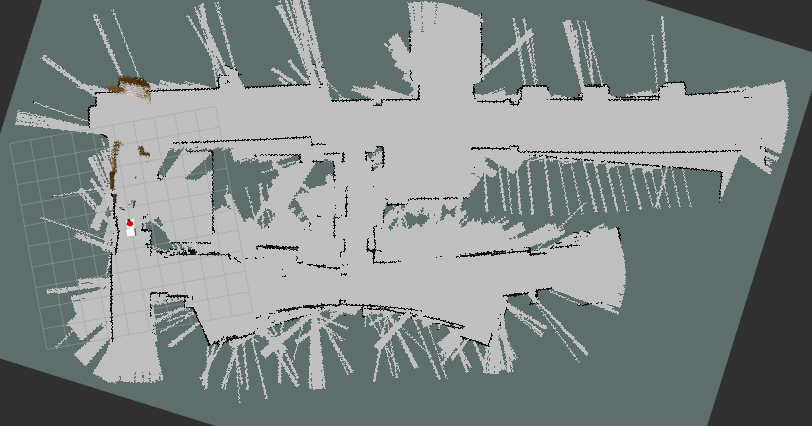
\includegraphics[width=\textwidth]{mapping_gamle_elektro}
		\caption{Resulting occupancy grid after a mapping session. The mapping  method is struggling with the  hallway in the upper part of the image.}
		\label{fig:mapping_gamle_elektro}
	\end{subfigure}
	\begin{subfigure}[b]{1\textwidth}
		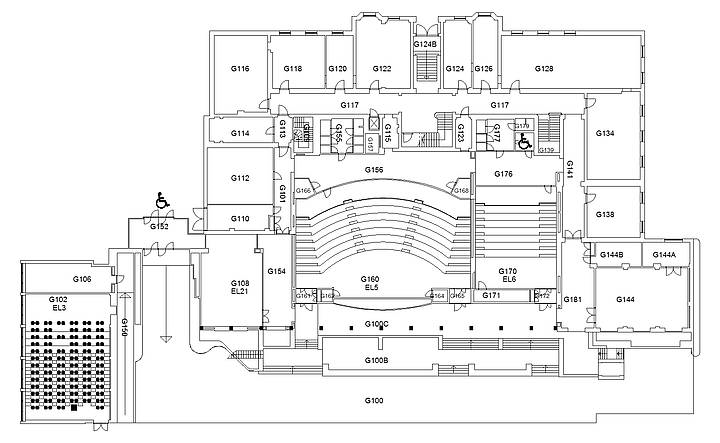
\includegraphics[width=\textwidth]{floorPlan}
		\caption{Floor plan of Gamle Elektro, first floor.}
		\label{fig:floorPlan}
	\end{subfigure}
	\caption{Comparison between mapped occupancy grid and floor plan.}\label{fig:comparison}
\end{figure}



\begin{figure}[h]
	\centering
	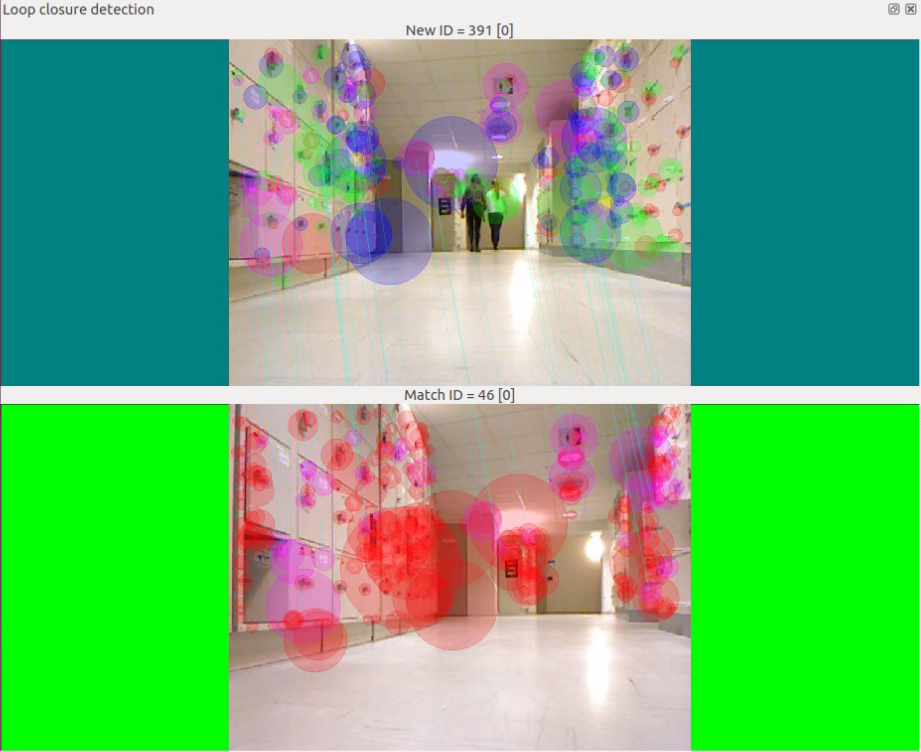
\includegraphics[width=1\textwidth]{lc_match_live}
	\caption{An example of an accepted loop closure hypothesis. This example is from the ''Asphalt'' world simulated in Gazebo.}
	\label{fig:lc_match_live}
\end{figure}

\begin{figure}[p]
	\centering
	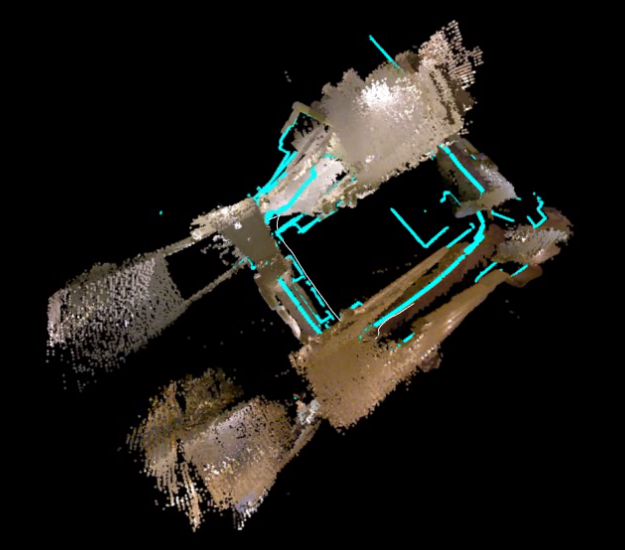
\includegraphics[width=1\textwidth]{lc_match_live_map}
	\caption{The resulting 3D map of the same area as in figure \ref{fig:mapping_gamle_elektro}.}
	\label{fig:lc_match_live_map}
\end{figure}

\subsubsection{Multi Session Mapping}

Multi session mapping was tested by performing an initial mapping run and then starting a second mapping session from an unknown location. All multi session mapping trials were successful. 

\subsubsection{Navigating Among Static Obstacles}

The first live navigation trials were performed by setting up a static obstacle course in a hallway. Only a few people were using this hallway, so multiple trials could be carried in under similar conditions. Most navigation trials were carried out in mapped areas. The robot performed well when navigating in known environments. In unknown environments, the robot will still plan a path. 



\subsubsection{Avoiding Moving Obstacles}

The navigation stack is configured to use a static global map for global planning and a local cost map that is linked with the mobile base and is based on real time sensor data. The local cost map will receive LIDAR laser scans, Kinect point clouds and point clouds representing detected obstacles detected by \texttt{rtabmap}. Being a real-time map, the local cost map should enable the local planner to avoid people and other non-static obstacles.

Moving obstacle avoidance testing was performed by having a person move into the planned path of the robot at different distances. Other avoidance situations would occur randomly as people were walking by the robot in the hallways. Tests showed that the robot is able to avoid non-static obstacles if the obstacle is observed at a distance larger than $0.5 - 0.8 m$. Figure \ref{fig:obstacle_avoidance} shows that the robot has successfully planned a new path around a person. If an obstacle appeared any closer than this, the new circumnavigating plan would either be too close to the original plan or not be planned at all. Detection and planning was not instantaneous. Some time would pass before the obstacle was detected and a new local plan was generated. This detection delay reduced the detectability of people walking by the robot. Figure \ref{fig:avoiding_moving_obstacles} shows an example of when the local cost map was lagging behind the actual moving obstacle.



\begin{figure}[p]
	\centering
	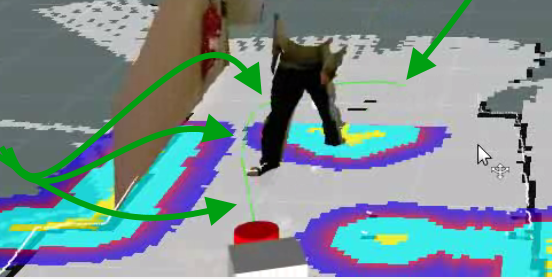
\includegraphics[width=1\textwidth]{avoiding_moving_obstacles_arrow}
	\caption{Avoiding moving obstacles with a new plan that circumnavigates the detected obstruction. In this situation, the obstacle was moving too fast for the local planner. The right leg is not yet registered as an obstacle.}
	\label{fig:avoiding_moving_obstacles}
\end{figure}

\begin{figure}
	\centering
	\begin{subfigure}[b]{0.46\textwidth}
		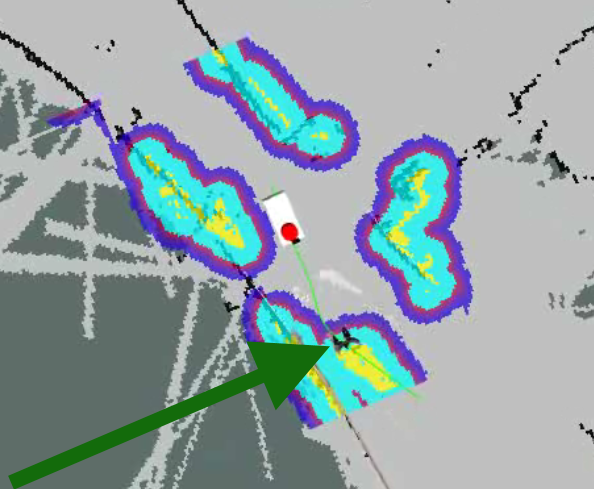
\includegraphics[width=\textwidth]{obstructed_plan_arrow}
		\caption{A person has moved into the path of the robot.}
		\label{fig:obstructed_plan}
	\end{subfigure}
	\begin{subfigure}[b]{0.472\textwidth}
		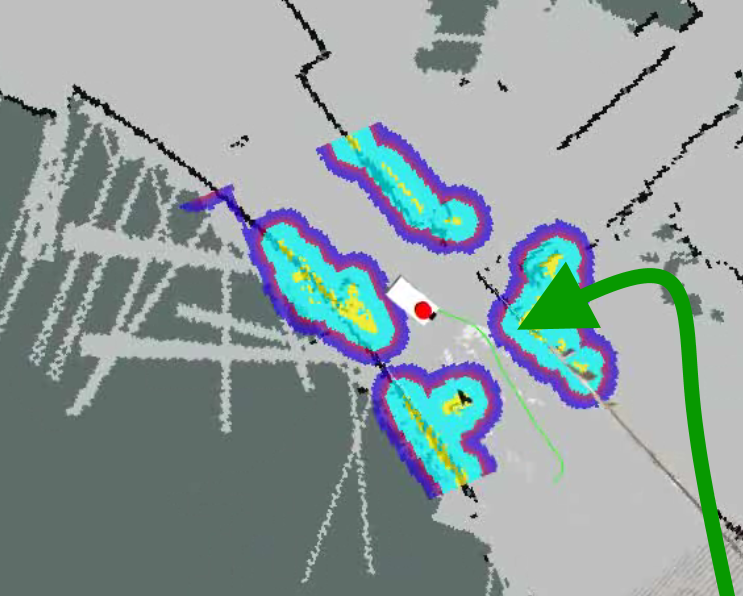
\includegraphics[width=\textwidth]{corrected_plan_arrow}
		\caption{A new path is planned, avoiding the new obstacle.}
		\label{fig:corrected_plan}
	\end{subfigure}
	\caption{Moving obstacle avoidance. The local cost map, shown as coloured spots on the occupancy grid, is based on real-time sensor data. }\label{fig:obstacle_avoidance}
\end{figure}




\section{Discussion}
\chapter{Discussion}
\label{chp:discussion} 

\section{Mapping}

\begin{itemize}
\item Repairing broken maps? What to do when map is partially broken.
\item Poor odometry when surrounding are in motion, or when laser features are difficult to detect. System can be fooled easily. 
\end{itemize}

\section{Navigation}
\begin{itemize}
\item Rectangle base vs. square base.
\item holonomic wheel.
\item Open loop wheel control (stuck when friction is high.)
\item Same as for mapping. Poor odometry when surrounding are in motion, or when laser features are difficult to detect. System can be fooled easily. 
\end{itemize}


\section{Suitability for Offshore Maintenance}

This is just a prototype. Mobility issues.
Kinect-like sensors and ROS could be useful. It is at least an excellent tool for ''rapid'' prototyping.

\subsection{Open Source Software and Security}

\ac{ROS} and other open source projects thrive on active communities of contributors. Both \ac{PCL} and \ac{ROS}, as well as many other libraries and frameworks, are built on a collaborative effort from researchers and developers across the globe. This is open structure is great for speeding up innovation. Issues and bugs can also be discovered more quickly by anyone. Another benefit is that every detail in an open source project is open for scrutiny by those who want to use it. This is also a problem in terms of security. While anyone can find bugs and issues, the code is also open to those who are looking for possible exploits and vulnerabilities. If a system is targeted for sabotage, and it is widely known that the system uses open source software, it might be more vulnerable to security threats.


\chapter{Conclusion}
\label{chp:conclusion} 

\section{Future Work}

\subsection{Autonomous Non-Destructive Testing}

Advancements in \ac{AI}, big data and machine learning opens up exciting possibilities for autonomous \ac{NDT}. Branches of this technology is usually encountered in the context of image recognition, i.e. teaching machines to understand what they see. The same concepts may be applied to forms of \ac{NDT} besides regular visual sensor input, such as ultra sound or eddy currents for corrosion detection.  

\subsection{Large Scale Kinect Fusion - Kintinous}

Kinect Fusion has great potential for augmented reality. Augmented reality is a concept which blends the real and virtual environment. This opens up opportunities to create realistic and immersive training scenarios for the operators. Unfortunately, Kinect Fusion is limited reconstructing a rather small volume depending on the resolution. By varying the resolution, volumes can at the least cover a normal office desk and at the most cover a small room \cite{keylist}.  

Kintinous...

A guide on how to build Kintinous can be found  at \href{Github}{https://github.com/mp3guy/Kintinuous}. The procedure is complicated, as it usually is for experimental builds. It is recommended to attempt the procedure on a fresh install of Ubuntu 14.04 or 15.04 \cite{Kintinous}.

\section{Task Fulfillment}

\section{Task Fulfilment}

\section{Final Conclusion}

\renewcommand*{\bibname}{References}
\bibliographystyle{alpha}
\bibliography{main}

%% Uncomment the following if you have any appendix
\appendix
 \addtocontents{toc}{%
  \protect\vspace{1em}% 
  \protect\noindent \bfseries \appendixtocname\protect\par
  \protect\vspace{-.5em}%
 }
 \renewcommand{\chaptername}{\appendixname}
%% include below possible appendices (chapters)
\chapter{Setting Up the Project}

\section{Hardware Setup}

For a guide on how to connect the hardware, consult figure \ref{fig:power} and \ref{fig:sensor_connections}. Otherwise, see the hardware list. A principal connection diagram for the network is shown in figure \ref{fig:network_setup}. The router should already be configured for communications. In not, consult \cite{aspunvik}.

\begin{figure}[h]
	\centering
	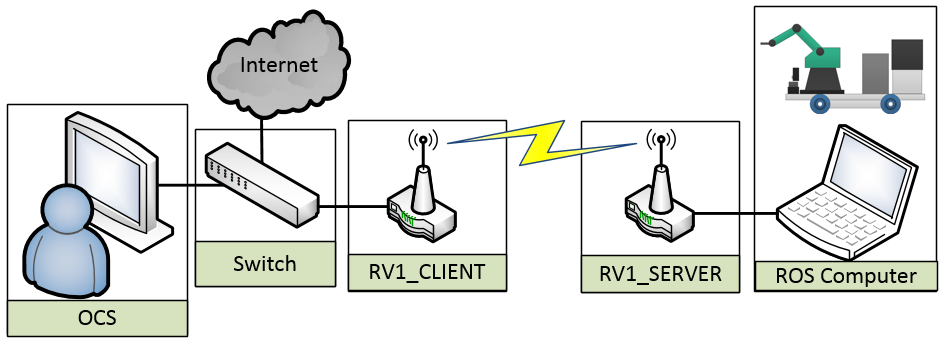
\includegraphics[width=0.85\textwidth]{network_setup}
	\caption{Network hardware setup. }
	\label{fig:network_setup}
\end{figure}

\subsubsection{Lead Battery Safety Precautions}

The lead battery used in this project (black 24V 48Ah, Biltema), is contains a large amount of energy and highly corrosive sulfuric acid. Remember to read the warning label, and Handle the battery with care. 

An explosive mix of hydrogen and oxygen may be formed when charging the battery. Some safety precautions are necessary to handle the risk:

\begin{itemize}
	\item Always charge the battery in a well ventilated area. 
	\item Turn the charger off before removing the connecting clamps.
	\item Allow some time to pass after charging before connecting or disconnecting cables to the battery poles.
\end{itemize} 

\subsubsection{Equipment List}
\begin{itemize}
	\item A computer that can be mounted on the robot. The computer must run on Linux Ubuntu (13.10 or 14.04 for ROS Indigo) and have a Bluetooth adapter.
	\item Two wireless routers (for example TP-Link).
	\item Two sinus inverters. One power inverter from Biltema and a silver colored pure sine inverter.
	\item One 12V Battery. The battery used in this project has a capacity of $45 Ah$.
	\item A $230V AC/24V DC$ converter.
	\item One XMEGA A3BU evalation board.
	\item One Hokuyo URG-04LX-UG01 LIDAR.
	\item A Kinect for XBOX 360 or an equivalent OpenNI depth camera.
\end{itemize}



\section{Installation}

\subsection{Software list}

This guide assumes that ROS Indigo is being used on a comparable system, for example Ubuntu 14.04. A guide for installing either ROS or Ubuntu is best aquired elsewhere. For ROS, see \url{ros.org}. Indigo was chosen primarily because of \texttt{openni\_launch}. 

\begin{description}
	\item[Hector SLAM for ROS] Install with \begin{verbatim} sudo apt-get install ros-indigo-hector-slam \end{verbatim}
	\item[Web video server node] Install with \begin{verbatim} sudo apt-get install ros-indigo-web-video-server \end{verbatim}
	\item[LIDAR driver] Install with \begin{verbatim} sudo apt-get install ros-indigo-hokuyo-node \end{verbatim}
	\item[RTAB-Map] Installed from source. Guide available at\\
	\url{https://github.com/introlab/rtabmap/wiki/Installation#ros}
	\item[Gazebo]  Install with \begin{verbatim} sudo apt-get install ros-indigo-gazebo-ros-pkgs \end{verbatim}
	Otherwise, consult \url{http://wiki.ros.org/gazebo_ros_pkgs}.
\end{description}

\section{Configuring the Project}

\subsection{Configuring the ROS Workspace}

Assuming that ROS is installed and properly configured, the first step in configuring the project is to create a catkin workspace. The custom ROS packages bundled with the digital attachments, should be placed in the \texttt{src} folder within the catkin workspace.

\subsection{Configuring the Bluetooth Connection}

The Qt framework is used to simplify the implementation of the Bluetooth connection between the \ac{ROS} graph and a remote device. Our \ac{ROS} installation for this project already includes some variant of Qt version 4.8. While useful for creating new \ac{GUI} applications, it lacks a Bluetooth API. The latest version of Qt, version 5.x, is equipped with libraries necessary for developing Bluetooth applications. This part of the guide will explain how to create a Qt 5 application which can be build by \texttt{catkin\_make} and run as a \textit{rosnode}.

\subsubsection{1 - Install Qt5}

Installing Qt5 for Linux is a straight forward procedure. Go to \url{qt.io}, and download the free version of Qt. All necessary instructions are provided. Qt5 may be installed in the home folder.

\subsubsection{2- Enabling Qt5 in a ROS node}

It is assumed that the \ac{ROS} package \texttt{bluetooth\_server}, is located in a catkin workspace:
\begin{verbatim}
	<NAME OF CATKIN WORKSPACE>/src/bluetooth_server
\end{verbatim}

Inside this folder, open the file ''CMakeLists.txt'' and locate the following:

\begin{verbatim}
set(CMAKE_PREFIX_PATH "/home/vegard/Qt/5.5/gcc_64/lib/cmake/Qt5"
					  "/home/vegard/Qt/5.5/gcc_64/lib/cmake/Qt5Core"
					  "/home/vegard/Qt/5.5/gcc_64/lib/cmake/Qt5Bluetooth"
\end{verbatim}

Change these paths to the correct paths on your system.

% FJERN DETTE DELKAPITTELET!
%\subsection{Adding the Qwt Plugin For Customizing QDial}

%This is a ''howto'' guide on how to install the Qwt-plugin.The following is assumed:

%\begin{itemize}
%	\item Development is performed on Windows 7
%	\item Qt 5.x is installed at c:/Qt
%\end{itemize}

\section{System Launch Procedure}

This procedure assumes that the \ac{ROS} implementation source code is placed in the \texttt{src} folder of a catkin workspace, and that he project has been built successfully. The first step is to go through a hardware checklist:

\begin{enumerate}
	\item Verify that the motor control board is connected to the wheel drivers, as shown in figure \ref{fig:conn_diag_motors}.
	\item Kinect, router and motors are connected to either internal or external power.
	\item Ensure that all USB ports are free. Exceptions apply to devices such as the Kinect or a mouse. 
	\item Connect the Hokuyo lidar (URG-04LX-UG01) to a USB port.
	\item Connect the motor control card to a USB port. Ensure that it is connected after the LIDAR. Ensure that the correct firmware is installed on the board.
\end{enumerate}

This procedure is recorded to video ''start\_live\_robot'': 

\begin{enumerate}
	\item Open five terminal windows.
	\item Launch \texttt{roscore} in one of the windows
	\item \texttt{cd} to \texttt{<your\_catkin\_workspace>/src/mar/scripts>}
	\item In this folder, run \texttt{\$ sudo ./setup\_hokuyo.sh}
	\item In the remaining three terminals, \texttt{cd} to your catkin workspace.
	\item In each of the terminals, run \texttt{\$ source ./devel/setup.bash}
	\item In one terminal, bring up the robot with\\ \texttt{\$ roslaunch mar mar\_bringup.launch}
	\item In another terminal, launch rtabmap with\\ \texttt{\$ roslaunch mar rtabmap.launch}\\
	Consult the launch file to see argument options.
	\item In the last terminal, launch navigation with\\ \texttt{\$ roslaunch mar\_2dnav move\_base.launch}
\end{enumerate}
\chapter{Troubleshooting}

\section{Introduction}

This part of the thesis contains answers to some of the problems that was encountered over the course od the semester. The solutions are not complete or comprehensive, but may provide some quick fixes for any students that may continue working with this project.

\section{Gazebo}

\subsection{\textcolor{red}{Error [Node.cc.90]} No namespace found}

\textbf{Solution: } Remember to source the \textit{gazebo} installation. In this case, with \textit{gazebo-2.2} installed as recommended for \ac{ROS} Indigo, the setup file can be sourced by entering

\begin{verbatim}
	$ source /usr/share/gazebo-2.2/setup.sh
\end{verbatim}

\subsection{Dependency Issues When Installing \textit{gazebo2}}

This problem was encountered after removing gazebo and then typing

\begin{verbatim}
$ sudo apt-get upgrade
\end{verbatim}

When typing 

\begin{verbatim}
$ sudo apt-get install -y gazebo2
\end{verbatim}

the installation failed because some dependencies had been upgraded to an incompatible version. To solve this, take note of the missing dependencies listed after entering the command above, open Ubuntu Software Center and select the History tab. Scroll down and locate the missing dependencies. They should have a red X next to them, indicating that they have been uninstalled. Then, enter the following command:

\begin{verbatim}
$ sudo apt-get install <NAME OF THE UNINSTALLED DEPENDENCY>
\end{verbatim}

\textit{gazebo2} 
\chapter{DVD Contents}
\label{chp:dvd_contents}



\begin{itemize}
	\item Master Thesis
	\item Project files: Robot (ROS)
	\item Project files: Operator Control Station (Qt)
	\item Project files: ''Robot Leash'' (Android)
	\item Project files: ''mar\_motor\_driver'' (C - Atmel)
	\item Videos
	\begin{itemize}
			\item live\_3d\_obstructions
			\item live\_first\_large\_scale\_mapping
			\item live\_mapping\_odom\_drift
			\item live\_mapping\_succesful
			\item live\_multi\_session\_mapping
			\item live\_navigation\_1
			\item live\_navigation\_2
			\item Obstruction detection and avoidance
			\item ocs\_test
			\item ocs\_test2
			\item sim\_global\_plan
			\item sim\_global\_plan\_poor\_localization
			\item sim\_wrong\_loop\_closure
			\item start\_live\_robot
	\end{itemize}
	\item Images

\end{itemize}


\end{document} 
